% Options for packages loaded elsewhere
\PassOptionsToPackage{unicode}{hyperref}
\PassOptionsToPackage{hyphens}{url}
\documentclass[
  american,
  11pt,
]{article}
\usepackage{xcolor}
\usepackage[margin=22mm]{geometry}
\usepackage{amsmath,amssymb}
\setcounter{secnumdepth}{-\maxdimen} % remove section numbering
\usepackage{iftex}
\ifPDFTeX
  \usepackage[T1]{fontenc}
  \usepackage[utf8]{inputenc}
  \usepackage{textcomp} % provide euro and other symbols
\else % if luatex or xetex
  \usepackage{fontspec} % this also loads fontspec
  \defaultfontfeatures{Scale=MatchLowercase}
  \defaultfontfeatures[\rmfamily]{Ligatures=TeX,Scale=1}
\fi
\usepackage{lmodern}
\ifPDFTeX\else
  % xetex/luatex font selection
  \setmainfont[]{Times New Roman}
  \setsansfont[]{Arial}
  \setmonofont[]{Consolas}
\fi
% Use upquote if available, for straight quotes in verbatim environments
\IfFileExists{upquote.sty}{\usepackage{upquote}}{}
\IfFileExists{microtype.sty}{% use microtype if available
  \usepackage[]{microtype}
  \UseMicrotypeSet[protrusion]{basicmath} % disable protrusion for tt fonts
}{}
\makeatletter
\@ifundefined{KOMAClassName}{% if non-KOMA class
  \IfFileExists{parskip.sty}{%
    \usepackage{parskip}
  }{% else
    \setlength{\parindent}{0pt}
    \setlength{\parskip}{6pt plus 2pt minus 1pt}}
}{% if KOMA class
  \KOMAoptions{parskip=half}}
\makeatother
\usepackage{listings}
\newcommand{\passthrough}[1]{#1}
\lstset{defaultdialect=[5.3]Lua}
\lstset{defaultdialect=[x86masm]Assembler}
\usepackage{longtable,booktabs,array}
\newcounter{none} % for unnumbered tables
\usepackage{calc} % for calculating minipage widths
% Correct order of tables after \paragraph or \subparagraph
\usepackage{etoolbox}
\makeatletter
\patchcmd\longtable{\par}{\if@noskipsec\mbox{}\fi\par}{}{}
\makeatother
% Allow footnotes in longtable head/foot
% No table footnotes.

\usepackage{graphicx}
\makeatletter
\newsavebox\pandoc@box
\newcommand*\pandocbounded[1]{% scales image to fit in text height/width
  \sbox\pandoc@box{#1}%
  \Gscale@div\@tempa{\textheight}{\dimexpr\ht\pandoc@box+\dp\pandoc@box\relax}%
  \Gscale@div\@tempb{\linewidth}{\wd\pandoc@box}%
  \ifdim\@tempb\p@<\@tempa\p@\let\@tempa\@tempb\fi% select the smaller of both
  \ifdim\@tempa\p@<\p@\scalebox{\@tempa}{\usebox\pandoc@box}%
  \else\usebox{\pandoc@box}%
  \fi%
}
% Set default figure placement to htbp
\def\fps@figure{htbp}
\makeatother
% definitions for citeproc citations
\NewDocumentCommand\citeproctext{}{}
\NewDocumentCommand\citeproc{mm}{%
  \begingroup\def\citeproctext{#2}\cite{#1}\endgroup}
\makeatletter
 % allow citations to break across lines
 \let\@cite@ofmt\@firstofone
 % avoid brackets around text for \cite:
 \def\@biblabel#1{}
 \def\@cite#1#2{{#1\if@tempswa , #2\fi}}
\makeatother
\newlength{\cslhangindent}
\setlength{\cslhangindent}{1.5em}
\newlength{\csllabelwidth}
\setlength{\csllabelwidth}{3em}
\newenvironment{CSLReferences}[2] % #1 hanging-indent, #2 entry-spacing
 {\begin{list}{}{%
  \setlength{\itemindent}{0pt}
  \setlength{\leftmargin}{0pt}
  \setlength{\parsep}{0pt}
  % turn on hanging indent if param 1 is 1
  \ifodd #1
   \setlength{\leftmargin}{\cslhangindent}
   \setlength{\itemindent}{-1\cslhangindent}
  \fi
  % set entry spacing
  \setlength{\itemsep}{#2\baselineskip}}}
 {\end{list}}
\usepackage{calc}
\newcommand{\CSLBlock}[1]{\hfill\break\parbox[t]{\linewidth}{\strut\ignorespaces#1\strut}}
\newcommand{\CSLLeftMargin}[1]{\parbox[t]{\csllabelwidth}{\strut#1\strut}}
\newcommand{\CSLRightInline}[1]{\parbox[t]{\linewidth - \csllabelwidth}{\strut#1\strut}}
\newcommand{\CSLIndent}[1]{\hspace{\cslhangindent}#1}
\ifLuaTeX
\usepackage[bidi=basic,shorthands=off]{babel}
\else
\usepackage[bidi=default,shorthands=off]{babel}
\fi
\ifPDFTeX
\else
\babelfont{rm}[]{Times New Roman}
\fi
\ifLuaTeX
  \usepackage{selnolig} % disable illegal ligatures
\fi
\setlength{\emergencystretch}{3em} % prevent overfull lines
\providecommand{\tightlist}{%
  \setlength{\itemsep}{0pt}\setlength{\parskip}{0pt}}

\usepackage{pdflscape}
\usepackage{etoolbox}
\usepackage{needspace}
\lstset{basicstyle=\ttfamily\footnotesize,breaklines=true,breakatwhitespace=false,
  columns=fullflexible,keepspaces=true,showstringspaces=false}
\AtBeginEnvironment{longtable}{\footnotesize}
\AtBeginEnvironment{CSLReferences}{\interlinepenalty=10000}
\setlength{\emergencystretch}{8em}
\widowpenalty=10000\clubpenalty=10000
\setlength{\LTpre}{6pt}\setlength{\LTpost}{6pt}
\setlength{\tabcolsep}{5.8pt}
\AtBeginDocument{\hypersetup{colorlinks=true,linkcolor=blue,urlcolor=blue,citecolor=blue}}
\usepackage{hyperref}
\IfFileExists{xurl.sty}{\usepackage{xurl}}{} % add URL line breaks if available
\urlstyle{same}
\hypersetup{
  pdftitle={Supplement: complete observations{,} mathematical comparisons and reproducibility},
  pdflang={en-US},
  hidelinks,
  pdfcreator={LaTeX via pandoc}}

\title{Supplement: complete observations, mathematical comparisons and
reproducibility}
\author{}
\date{14 November 2026}

\begin{document}
\maketitle

{
\setcounter{tocdepth}{2}
\tableofcontents
}
The current tables contain every registered position. C means a
performance-eligible qualified certificate; O means open; UEV means
evidence outside formal performance eligibility. Open times are null,
not the cap. Detailed full-precision arrays, physical operations, raw
lifecycle/model evidence and source identities accompany the CSV/JSON
authorities. Prior evidence below keeps its original version and
denominators.

\subsection{Reading and source map}\label{reading-and-source-map}

The main paper and complete model/algorithm appendices are assembled
from \texttt{paper\_\allowbreak{}body.md} and
\texttt{model\_\allowbreak{}and\_\allowbreak{}algorithm\_\allowbreak{}appendices.md}. This
supplement keeps complete breadth/resource/weight/AM/mechanism
observations, useful historical mathematical comparisons, source
provenance and the later cohort evidence. The
\href{https://github.com/yifanXovo/TailoredExact/blob/codex/round166-structure-and-paper/results/unified_exact_round137/mathematical_analysis.md}{mathematical
companion} distinguishes the relaxation objects and proof contracts. The
\href{https://github.com/yifanXovo/TailoredExact/blob/codex/round166-structure-and-paper/results/unified_exact_round166/source_manifest.json}{current
source manifest} and
\href{https://github.com/yifanXovo/TailoredExact/blob/codex/round166-structure-and-paper/results/unified_exact_round166/document_build.json}{document
build receipt} bind the current PDF to those components. Administrative
author decisions are kept in the internal memo and are not part of the
technical manuscript.

\subsection{Current detailed panel
tables}\label{current-detailed-panel-tables}

Complete panel observations accompany the compact question-led main
text. Shared defaults retain their actual position identities.

\Needspace{358pt}

\subsection{Breadth: complete two-sided
endpoints}\label{breadth-complete-two-sided-endpoints}

{\def\LTcaptype{none} % do not increment counter
\begin{longtable}[]{@{}
  >{\raggedright\arraybackslash}p{(\linewidth - 6\tabcolsep) * \real{0.2500}}
  >{\raggedright\arraybackslash}p{(\linewidth - 6\tabcolsep) * \real{0.2500}}
  >{\raggedright\arraybackslash}p{(\linewidth - 6\tabcolsep) * \real{0.2500}}
  >{\raggedright\arraybackslash}p{(\linewidth - 6\tabcolsep) * \real{0.2500}}@{}}
\toprule\noalign{}
\begin{minipage}[b]{\linewidth}\raggedright
Input
\end{minipage} & \begin{minipage}[b]{\linewidth}\raggedright
P: U / L
\end{minipage} & \begin{minipage}[b]{\linewidth}\raggedright
PS: U / L
\end{minipage} & \begin{minipage}[b]{\linewidth}\raggedright
GI-TBC: U / L
\end{minipage} \\
\midrule\noalign{}
\endhead
\bottomrule\noalign{}
\endlastfoot
K-15-S & 0.592265 / 0.527663 & 0.592265 / 0.520583 & 0.592265 /
0.592265 \\
X-15-B & 0 / 0 & 0 / 0 & 0 / 0 \\
UC-B20-B & 0.577333 / 0.577333 & 0.577333 / 0.577333 & 0.577333 /
0.577333 \\
K-20-S & 0.727702 / 0.541868 & 0.775213 / 0.541233 & 0.716807 /
0.705356 \\
K-35-U & 0.664747 / 0.335556 & 0.767457 / 0.331922 & 0.692854 /
0.565766 \\
X-35-B & 0 / 0 & 0 / 0 & 0 / 0 \\
N-B15-B & 0.250494 / 0.250494 & 0.250494 / 0.250494 & 0.250494 /
0.250494 \\
N-X15-S & 0.628986 / 0.628986 & 0.628986 / 0.628986 & 0.628986 /
0.628986 \\
N-C20-U & 0.248551 / 0.217719 & 0.252309 / 0.214733 & 0.245505 /
0.245505 \\
N-X20-B & 0 / 0 & 0 / 0 & 0 / 0 \\
N-B35-S & 0.844874 / 0.371908 & 0.486013 / 0.373343 & 0.450292 /
0.389311 \\
N-C35-B & 0 / 0 & 0 / 0 & 0 / 0 \\
\end{longtable}
}

\Needspace{270pt}

\subsection{Positive-resource GI-TBC operating
points}\label{positive-resource-gi-tbc-operating-points}

{\def\LTcaptype{none} % do not increment counter
\begin{longtable}[]{@{}
  >{\raggedright\arraybackslash}p{(\linewidth - 8\tabcolsep) * \real{0.2000}}
  >{\raggedright\arraybackslash}p{(\linewidth - 8\tabcolsep) * \real{0.2000}}
  >{\raggedright\arraybackslash}p{(\linewidth - 8\tabcolsep) * \real{0.2000}}
  >{\raggedright\arraybackslash}p{(\linewidth - 8\tabcolsep) * \real{0.2000}}
  >{\raggedright\arraybackslash}p{(\linewidth - 8\tabcolsep) * \real{0.2000}}@{}}
\toprule\noalign{}
\begin{minipage}[b]{\linewidth}\raggedright
Configuration
\end{minipage} & \begin{minipage}[b]{\linewidth}\raggedright
G / \(P_{\mathrm{avg}}\) / S
\end{minipage} & \begin{minipage}[b]{\linewidth}\raggedright
Returned units
\end{minipage} & \begin{minipage}[b]{\linewidth}\raggedright
Max duration / T
\end{minipage} & \begin{minipage}[b]{\linewidth}\raggedright
Status
\end{minipage} \\
\midrule\noalign{}
\endhead
\bottomrule\noalign{}
\endlastfoot
R-B20-S-T1 & 0.216444 /0.264291 /17.2599 & 0 & 0.999851 & C \\
R-B20-S-T2 & 0.0819181 /0.116555 /17.4317 & 0 & 0.999816 & C \\
R-X20-S-T1 & 0.314652 /0.330673 /14.5762 & 1 & 0.999834 & C \\
R-X20-S-T2 & 0.206001 /0.228795 /15.7226 & 0 & 0.997641 & C \\
R-B35-S-T1 & 0.285367 /0.30615 /29.2099 & 2 & 0.994109 & open \\
R-B35-S-T2 & 0.181545 /0.163098 /29.8127 & 3 & 0.996291 & open \\
R-X35-S-T1 & 0.268135 /0.324055 /28.7591 & 1 & 0.999456 & open \\
R-X35-S-T2 & 0.18255 /0.220722 /28.2238 & 0 & 0.998568 & open \\
\end{longtable}
}

\begin{landscape}

\subsection{Objective weights: all methods and
decompositions}\label{objective-weights-all-methods-and-decompositions}

{\def\LTcaptype{none} % do not increment counter
\begin{longtable}[]{@{}
  >{\raggedright\arraybackslash}p{(\linewidth - 10\tabcolsep) * \real{0.1667}}
  >{\raggedright\arraybackslash}p{(\linewidth - 10\tabcolsep) * \real{0.1667}}
  >{\raggedright\arraybackslash}p{(\linewidth - 10\tabcolsep) * \real{0.1667}}
  >{\raggedright\arraybackslash}p{(\linewidth - 10\tabcolsep) * \real{0.1667}}
  >{\raggedright\arraybackslash}p{(\linewidth - 10\tabcolsep) * \real{0.1667}}
  >{\raggedright\arraybackslash}p{(\linewidth - 10\tabcolsep) * \real{0.1667}}@{}}
\toprule\noalign{}
\begin{minipage}[b]{\linewidth}\raggedright
Configuration
\end{minipage} & \begin{minipage}[b]{\linewidth}\raggedright
\(\rho\)
\end{minipage} & \begin{minipage}[b]{\linewidth}\raggedright
Method
\end{minipage} & \begin{minipage}[b]{\linewidth}\raggedright
G / \(P_{\mathrm{avg}}\)
\end{minipage} & \begin{minipage}[b]{\linewidth}\raggedright
U / L
\end{minipage} & \begin{minipage}[b]{\linewidth}\raggedright
Certificate
\end{minipage} \\
\midrule\noalign{}
\endhead
\bottomrule\noalign{}
\endlastfoot
R-B20-S-T1 & 1 & P & 0.239416 / 0.300668 & 0.540085 / 0.358158 & open \\
R-B20-S-T1 & 1 & PS & 0.222348 / 0.264291 & 0.486639 / 0.365324 &
open \\
R-B20-S-T1 & 1 & GI-TBC & 0.216444 / 0.264291 & 0.480735 / 0.480735 &
C \\
R-X35-S-T2 & 1 & PS & 0.194085 / 0.210482 & 0.404567 / 0.203817 &
open \\
R-X35-S-T2 & 1 & GI-TBC & 0.18255 / 0.220722 & 0.403272 / 0.210887 &
open \\
R-X35-S-T2 & 1 & P & 0.205654 / 0.284863 & 0.490517 / 0.201288 & open \\
R-B20-S-T1 & 0.5 & P & 0.223002 / 0.314774 & 0.380389 / 0.229542 &
open \\
R-B20-S-T1 & 0.5 & PS & 0.213456 / 0.268003 & 0.347458 / 0.240479 &
open \\
R-B20-S-T1 & 0.5 & GI-TBC & 0.213456 / 0.268003 & 0.347458 / 0.331864 &
open \\
R-B20-S-T1 & 2 & P & 0.232861 / 0.262064 & 0.756988 / 0.610312 & open \\
R-B20-S-T1 & 2 & PS & 0.217549 / 0.263549 & 0.744646 / 0.616106 &
open \\
R-B20-S-T1 & 2 & GI-TBC & 0.217549 / 0.263549 & 0.744646 / 0.744646 &
C \\
R-X35-S-T2 & 0.5 & PS & 0.136611 / 0.242041 & 0.257631 / 0.108019 &
open \\
R-X35-S-T2 & 0.5 & GI-TBC & 0.137132 / 0.237386 & 0.255825 / 0.122332 &
open \\
R-X35-S-T2 & 0.5 & P & 0.141354 / 0.239248 & 0.260978 / 0.108223 &
open \\
R-X35-S-T2 & 2 & PS & 0.198468 / 0.206712 & 0.611892 / 0.363572 &
open \\
R-X35-S-T2 & 2 & GI-TBC & 0.148459 / 0.188047 & 0.524553 / 0.388438 &
open \\
R-X35-S-T2 & 2 & P & 0.203202 / 0.20862 & 0.620443 / 0.36178 & open \\
\end{longtable}
}

\end{landscape}

\begin{landscape}

\subsection{Limited Seed 1: complete main
triplets}\label{limited-seed-1-complete-main-triplets}

{\def\LTcaptype{none} % do not increment counter
\begin{longtable}[]{@{}
  >{\raggedright\arraybackslash}p{(\linewidth - 10\tabcolsep) * \real{0.1667}}
  >{\raggedright\arraybackslash}p{(\linewidth - 10\tabcolsep) * \real{0.1667}}
  >{\raggedright\arraybackslash}p{(\linewidth - 10\tabcolsep) * \real{0.1667}}
  >{\raggedright\arraybackslash}p{(\linewidth - 10\tabcolsep) * \real{0.1667}}
  >{\raggedright\arraybackslash}p{(\linewidth - 10\tabcolsep) * \real{0.1667}}
  >{\raggedright\arraybackslash}p{(\linewidth - 10\tabcolsep) * \real{0.1667}}@{}}
\toprule\noalign{}
\begin{minipage}[b]{\linewidth}\raggedright
Role
\end{minipage} & \begin{minipage}[b]{\linewidth}\raggedright
Method
\end{minipage} & \begin{minipage}[b]{\linewidth}\raggedright
Status
\end{minipage} & \begin{minipage}[b]{\linewidth}\raggedright
Own \(T_{\mathrm{cert}}\) (s)
\end{minipage} & \begin{minipage}[b]{\linewidth}\raggedright
U / L
\end{minipage} & \begin{minipage}[b]{\linewidth}\raggedright
Production (s)
\end{minipage} \\
\midrule\noalign{}
\endhead
\bottomrule\noalign{}
\endlastfoot
K-15-S & P & open & n/a & 0.592265 /0.529115 & 571.412 \\
K-15-S & PS & open & n/a & 0.592265 /0.53228 & 571.362 \\
K-15-S & GI-TBC & C & 115.444 & 0.592265 /0.592265 & 115.444 \\
R-B20-S-T1 & P & open & n/a & 0.493224 /0.354626 & 1171.09 \\
R-B20-S-T1 & PS & open & n/a & 0.480735 /0.367482 & 1171.18 \\
R-B20-S-T1 & GI-TBC & C & 656.734 & 0.480735 /0.480735 & 656.734 \\
UC-B20-B & P & C & 314.513 & 0.577333 /0.577333 & 314.513 \\
UC-B20-B & PS & C & 125.391 & 0.577333 /0.577333 & 125.391 \\
UC-B20-B & GI-TBC & C & 4.0999 & 0.577333 /0.577333 & 4.0999 \\
K-35-U & P & open & n/a & 0.758852 /0.330574 & 2371.17 \\
K-35-U & PS & open & n/a & 0.712648 /0.335095 & 2371.03 \\
K-35-U & GI-TBC & open & n/a & 0.668358 /0.55478 & 2371 \\
\end{longtable}
}

\end{landscape}

\Needspace{226pt}

\subsection{Limited Seed 1 AM
observations}\label{limited-seed-1-am-observations}

\textbf{Seed 1 limited AM repeat}

{\def\LTcaptype{none} % do not increment counter
\begin{longtable}[]{@{}
  >{\raggedright\arraybackslash}p{(\linewidth - 8\tabcolsep) * \real{0.2000}}
  >{\raggedright\arraybackslash}p{(\linewidth - 8\tabcolsep) * \real{0.2000}}
  >{\raggedright\arraybackslash}p{(\linewidth - 8\tabcolsep) * \real{0.2000}}
  >{\raggedright\arraybackslash}p{(\linewidth - 8\tabcolsep) * \real{0.2000}}
  >{\raggedright\arraybackslash}p{(\linewidth - 8\tabcolsep) * \real{0.2000}}@{}}
\toprule\noalign{}
\begin{minipage}[b]{\linewidth}\raggedright
Role
\end{minipage} & \begin{minipage}[b]{\linewidth}\raggedright
\(\tau_{\mathrm{AM}}\)
\end{minipage} & \begin{minipage}[b]{\linewidth}\raggedright
Max gate score
\end{minipage} & \begin{minipage}[b]{\linewidth}\raggedright
Actions
\end{minipage} & \begin{minipage}[b]{\linewidth}\raggedright
Production (s)
\end{minipage} \\
\midrule\noalign{}
\endhead
\bottomrule\noalign{}
\endlastfoot
K-15-S & 0.04 & 0.000356687 & native-target:1, exact-close:1 &
114.938 \\
K-15-S & 0.08 & 0.000356687 & native-target:1, exact-close:1 &
115.444 \\
K-15-S & 0.16 & 0.000356687 & native-target:1, exact-close:1 &
115.503 \\
UC-B20-B & 0.04 & 0.00031863 & split:3, native-target:1, exact-close:1 &
4.08256 \\
UC-B20-B & 0.08 & 0.00031863 & split:3, native-target:1, exact-close:1 &
4.0999 \\
UC-B20-B & 0.16 & 0.00031863 & split:3, native-target:1, exact-close:1 &
4.0657 \\
\end{longtable}
}

\subsection{Seed 0 main mechanism
comparison}\label{seed-0-main-mechanism-comparison}

{\def\LTcaptype{none} % do not increment counter
\begin{longtable}[]{@{}lllll@{}}
\toprule\noalign{}
Contrast & Role & Root LP optimum & Production (s) & Status \\
\midrule\noalign{}
\endhead
\bottomrule\noalign{}
\endlastfoot
GI-TBC & K-15-S & 0.167137 & 112.769 & C \\
GI-TBC-R & K-15-S & 0.167137 & 112.649 & C \\
minus A/B & K-15-S & 0.167016 & 128.325 & C \\
minus \(C_R\) & K-15-S & 0.167137 & 75.1064 & C \\
minus \(C_G\) & K-15-S & 0.167137 & 143.15 & C \\
GI-TBC & UC-B20-B & 0.479076 & 4.14897 & C \\
GI-TBC-R & UC-B20-B & 0.479076 & 1.87206 & C \\
minus A/B & UC-B20-B & 0.479076 & 4.18619 & C \\
minus \(C_R\) & UC-B20-B & 0.479076 & 4.91775 & C \\
minus \(C_G\) & UC-B20-B & 0.479076 & 3.34912 & C \\
GI-TBC & K-20-S & 0.195149 & 1172.19 & open \\
GI-TBC-R & K-20-S & 0.195149 & 1172.22 & open \\
minus A/B & K-20-S & 0.193825 & 1172.12 & open \\
minus \(C_R\) & K-20-S & 0.195149 & 1171.91 & open \\
minus \(C_G\) & K-20-S & 0.195149 & 1171.96 & open \\
GI-TBC & K-35-U & 0.200178 & 2371.15 & open \\
GI-TBC-R & K-35-U & 0.200178 & 2370.99 & open \\
minus A/B & K-35-U & 0.200178 & 2372.38 & open \\
minus \(C_R\) & K-35-U & 0.200178 & 2370.97 & open \\
minus \(C_G\) & K-35-U & 0.200178 & 2370.98 & open \\
\end{longtable}
}

\Needspace{314pt}

\subsection{Seed 1 limited mechanism
repeat}\label{seed-1-limited-mechanism-repeat}

{\def\LTcaptype{none} % do not increment counter
\begin{longtable}[]{@{}lllll@{}}
\toprule\noalign{}
Contrast & Role & Root LP optimum & Production (s) & Status \\
\midrule\noalign{}
\endhead
\bottomrule\noalign{}
\endlastfoot
GI-TBC & K-15-S & 0.167137 & 115.444 & C \\
GI-TBC-R & K-15-S & 0.167137 & 113.58 & C \\
minus A/B & K-15-S & 0.167016 & 93.6997 & C \\
minus \(C_R\) & K-15-S & 0.167137 & 132.475 & C \\
minus \(C_G\) & K-15-S & 0.167137 & 99.6006 & C \\
GI-TBC & UC-B20-B & 0.479076 & 4.0999 & C \\
GI-TBC-R & UC-B20-B & 0.479076 & 1.95408 & C \\
minus A/B & UC-B20-B & 0.479076 & 4.46646 & C \\
minus \(C_R\) & UC-B20-B & 0.479076 & 4.60284 & C \\
minus \(C_G\) & UC-B20-B & 0.479076 & 2.95877 & C \\
\end{longtable}
}

\begin{landscape}

{\def\LTcaptype{none} % do not increment counter
\begin{longtable}[]{@{}
  >{\raggedright\arraybackslash}p{(\linewidth - 12\tabcolsep) * \real{0.1429}}
  >{\raggedright\arraybackslash}p{(\linewidth - 12\tabcolsep) * \real{0.1429}}
  >{\raggedright\arraybackslash}p{(\linewidth - 12\tabcolsep) * \real{0.1429}}
  >{\raggedright\arraybackslash}p{(\linewidth - 12\tabcolsep) * \real{0.1429}}
  >{\raggedright\arraybackslash}p{(\linewidth - 12\tabcolsep) * \real{0.1429}}
  >{\raggedright\arraybackslash}p{(\linewidth - 12\tabcolsep) * \real{0.1429}}
  >{\raggedright\arraybackslash}p{(\linewidth - 12\tabcolsep) * \real{0.1429}}@{}}
\toprule\noalign{}
\begin{minipage}[b]{\linewidth}\raggedright
Position / study
\end{minipage} & \begin{minipage}[b]{\linewidth}\raggedright
Input / Seed
\end{minipage} & \begin{minipage}[b]{\linewidth}\raggedright
Method
\end{minipage} & \begin{minipage}[b]{\linewidth}\raggedright
Status
\end{minipage} & \begin{minipage}[b]{\linewidth}\raggedright
U
\end{minipage} & \begin{minipage}[b]{\linewidth}\raggedright
L
\end{minipage} & \begin{minipage}[b]{\linewidth}\raggedright
Production / verification / total s
\end{minipage} \\
\midrule\noalign{}
\endhead
\bottomrule\noalign{}
\endlastfoot
1 /B1 & K-15-S /0 & P & O & 0.592265 & 0.527663 & 571.702 /142.568
/714.27 \\
2 /B1 & K-15-S /0 & PS & O & 0.592265 & 0.520583 & 571.245 /2.27522
/573.52 \\
3 /B1 & K-15-S /0 & GI-TBC & C & 0.592265 & 0.592265 & 112.769 /3.77037
/116.54 \\
4 /B1 & X-15-B /0 & PS & C & 0 & 0 & 2.46104 /0.365936 /2.82698 \\
5 /B1 & X-15-B /0 & GI-TBC & C & 0 & 0 & 2.55662 /0.645774 /3.2024 \\
6 /B1 & X-15-B /0 & P & C & 0 & 0 & 7.0233 /0.248991 /7.2723 \\
7 /B1 & UC-B20-B /0 & GI-TBC & C & 0.577333 & 0.577333 & 4.14897 /2.347
/6.49597 \\
8 /B1 & UC-B20-B /0 & P & C & 0.577333 & 0.577333 & 315.403 /1.24106
/316.644 \\
9 /B1 & UC-B20-B /0 & PS & C & 0.577333 & 0.577333 & 236.091 /1.30849
/237.399 \\
10 /B1 & K-20-S /0 & P & O & 0.727702 & 0.541868 & 1171.16 /1.44439
/1172.61 \\
11 /B1 & K-20-S /0 & PS & O & 0.775213 & 0.541233 & 1171.21 /1.5361
/1172.74 \\
12 /B1 & K-20-S /0 & GI-TBC & O & 0.716807 & 0.705356 & 1172.19 /61.1438
/1233.33 \\
13 /B1 & K-35-U /0 & PS & O & 0.767457 & 0.331922 & 2371 /1.72964
/2372.73 \\
14 /B1 & K-35-U /0 & GI-TBC & O & 0.692854 & 0.565766 & 2371.15 /3.80005
/2374.95 \\
15 /B1 & K-35-U /0 & P & O & 0.664747 & 0.335556 & 2371.06 /0.722418
/2371.78 \\
16 /B1 & X-35-B /0 & GI-TBC & C & 0 & 0 & 17.9046 /3.63609 /21.5407 \\
17 /B1 & X-35-B /0 & P & C & 0 & 0 & 158.585 /0.596178 /159.181 \\
18 /B1 & X-35-B /0 & PS & C & 0 & 0 & 7.45014 /1.38966 /8.8398 \\
19 /B1 & N-B15-B /0 & P & C & 0.250494 & 0.250494 & 279.663 /1.67388
/281.337 \\
20 /B1 & N-B15-B /0 & PS & C & 0.250494 & 0.250494 & 306.307 /1.67192
/307.979 \\
21 /B1 & N-B15-B /0 & GI-TBC & C & 0.250494 & 0.250494 & 24.0684
/0.790358 /24.8587 \\
22 /B1 & N-X15-S /0 & PS & C & 0.628986 & 0.628986 & 401.931 /3.09583
/405.027 \\
23 /B1 & N-X15-S /0 & GI-TBC & C & 0.628986 & 0.628986 & 10.2683
/0.739441 /11.0077 \\
24 /B1 & N-X15-S /0 & P & C & 0.628986 & 0.628986 & 538.867 /3.46182
/542.329 \\
25 /B1 & N-C20-U /0 & GI-TBC & C & 0.245505 & 0.245505 & 265.529
/4.06871 /269.598 \\
26 /B1 & N-C20-U /0 & P & O & 0.248551 & 0.217719 & 1171.18 /1.83559
/1173.01 \\
27 /B1 & N-C20-U /0 & PS & O & 0.252309 & 0.214733 & 1171.14 /11.7494
/1182.89 \\
28 /B1 & N-X20-B /0 & P & C & 0 & 0 & 24.0892 /0.306578 /24.3958 \\
29 /B1 & N-X20-B /0 & PS & C & 0 & 0 & 6.08515 /0.486901 /6.57205 \\
30 /B1 & N-X20-B /0 & GI-TBC & C & 0 & 0 & 7.45537 /1.0786 /8.53397 \\
31 /B1 & N-B35-S /0 & PS & O & 0.486013 & 0.373343 & 2371.01 /1.74441
/2372.76 \\
32 /B1 & N-B35-S /0 & GI-TBC & O & 0.450292 & 0.389311 & 2370.98
/3.84726 /2374.82 \\
33 /B1 & N-B35-S /0 & P & O & 0.844874 & 0.371908 & 2371.11 /0.661396
/2371.77 \\
34 /B1 & N-C35-B /0 & GI-TBC & C & 0 & 0 & 59.6234 /3.71224 /63.3357 \\
35 /B1 & N-C35-B /0 & P & C & 0 & 0 & 397.807 /0.653354 /398.461 \\
36 /B1 & N-C35-B /0 & PS & C & 0 & 0 & 154.668 /1.42879 /156.097 \\
37 /B2 & R-B20-S-T1 /0 & P & O & 0.540085 & 0.358158 & 1171.18 /0.980204
/1172.16 \\
38 /B2 & R-B20-S-T1 /0 & PS & O & 0.486639 & 0.365324 & 1171.29 /1.3497
/1172.64 \\
39 /B2 & R-B20-S-T1 /0 & GI-TBC & C & 0.480735 & 0.480735 & 784.143
/18.1789 /802.322 \\
40 /B2 & R-B20-S-T2 /0 & PS & O & 0.208465 & 0.146203 & 1171.14 /1.19298
/1172.33 \\
41 /B2 & R-B20-S-T2 /0 & GI-TBC & C & 0.198473 & 0.198473 & 538.603
/5.73802 /544.341 \\
42 /B2 & R-B20-S-T2 /0 & P & O & 0.269095 & 0.141262 & 1171.19 /0.766113
/1171.96 \\
43 /B2 & R-X20-S-T1 /0 & GI-TBC & C & 0.645325 & 0.645325 & 20.5065
/1.08205 /21.5885 \\
44 /B2 & R-X20-S-T1 /0 & P & O & 0.645325 & 0.589197 & 1171.57 /5.00163
/1176.57 \\
45 /B2 & R-X20-S-T1 /0 & PS & O & 0.645325 & 0.590359 & 1171.69 /4.9291
/1176.62 \\
46 /B2 & R-X20-S-T2 /0 & P & O & 0.476731 & 0.291101 & 1171.1 /0.410932
/1171.51 \\
47 /B2 & R-X20-S-T2 /0 & PS & O & 0.51972 & 0.28447 & 1171.18 /0.839506
/1172.02 \\
48 /B2 & R-X20-S-T2 /0 & GI-TBC & C & 0.434796 & 0.434796 & 337.305
/2.72864 /340.034 \\
49 /B2 & R-B35-S-T1 /0 & PS & O & 0.631765 & 0.334519 & 2371.04 /1.73506
/2372.77 \\
50 /B2 & R-B35-S-T1 /0 & GI-TBC & O & 0.591518 & 0.455904 & 2376.07
/5.60112 /2381.67 \\
51 /B2 & R-B35-S-T1 /0 & P & O & 0.606311 & 0.337002 & 2372.2 /0.733367
/2372.93 \\
52 /B2 & R-B35-S-T2 /0 & GI-TBC & O & 0.344643 & 0.218986 & 2371.04
/3.76611 /2374.8 \\
53 /B2 & R-B35-S-T2 /0 & P & O & 0.471637 & 0.154376 & 2371.07 /0.692204
/2371.77 \\
54 /B2 & R-B35-S-T2 /0 & PS & O & 0.438291 & 0.155416 & 2371.03 /1.71384
/2372.75 \\
55 /B2 & R-X35-S-T1 /0 & P & O & 0.655713 & 0.296009 & 2371.09 /0.694498
/2371.79 \\
56 /B2 & R-X35-S-T1 /0 & PS & O & 0.593231 & 0.298839 & 2371.01 /4.60794
/2375.62 \\
57 /B2 & R-X35-S-T1 /0 & GI-TBC & O & 0.59219 & 0.463358 & 2379.12
/3.67396 /2382.79 \\
58 /B2 & R-X35-S-T2 /0 & PS & O & 0.404567 & 0.203817 & 2370.99 /1.72903
/2372.71 \\
59 /B2 & R-X35-S-T2 /0 & GI-TBC & O & 0.403272 & 0.210887 & 2371.09
/3.72914 /2374.82 \\
60 /B2 & R-X35-S-T2 /0 & P & O & 0.490517 & 0.201288 & 2371.02 /0.664748
/2371.68 \\
61 /B3 & R-B20-S-T1-rho0.5 /0 & P & O & 0.380389 & 0.229542 & 1171.17
/0.87512 /1172.05 \\
62 /B3 & R-B20-S-T1-rho0.5 /0 & PS & O & 0.347458 & 0.240479 & 1171.16
/1.17614 /1172.33 \\
63 /B3 & R-B20-S-T1-rho0.5 /0 & GI-TBC & O & 0.347458 & 0.331864 &
1171.29 /5.89166 /1177.18 \\
64 /B3 & R-B20-S-T1-rho2 /0 & P & O & 0.756988 & 0.610312 & 1171.15
/1.29992 /1172.45 \\
65 /B3 & R-B20-S-T1-rho2 /0 & PS & O & 0.744646 & 0.616106 & 1171.34
/1.7534 /1173.1 \\
66 /B3 & R-B20-S-T1-rho2 /0 & GI-TBC & C & 0.744646 & 0.744646 & 309.113
/8.59128 /317.704 \\
67 /B3 & R-X35-S-T2-rho0.5 /0 & PS & O & 0.257631 & 0.108019 & 2371.05
/1.73565 /2372.78 \\
68 /B3 & R-X35-S-T2-rho0.5 /0 & GI-TBC & O & 0.255825 & 0.122332 &
2371.1 /3.68103 /2374.78 \\
69 /B3 & R-X35-S-T2-rho0.5 /0 & P & O & 0.260978 & 0.108223 & 2371.1
/0.679667 /2371.78 \\
70 /B3 & R-X35-S-T2-rho2 /0 & PS & O & 0.611892 & 0.363572 & 2371.03
/1.71701 /2372.74 \\
71 /B3 & R-X35-S-T2-rho2 /0 & GI-TBC & O & 0.524553 & 0.388438 & 2370.96
/3.7818 /2374.74 \\
72 /B3 & R-X35-S-T2-rho2 /0 & P & O & 0.620443 & 0.36178 & 2371.09
/0.700077 /2371.79 \\
73 /C1 & K-15-S /0 & AM .04 & C & 0.592265 & 0.592265 & 113.062 /3.77321
/116.835 \\
74 /C1 & K-15-S /0 & AM .16 & C & 0.592265 & 0.592265 & 113.315 /3.74081
/117.056 \\
75 /C1 & K-20-S /0 & AM .04 & O & 0.716807 & 0.705366 & 1172.26 /61.3126
/1233.57 \\
76 /C1 & K-20-S /0 & AM .16 & O & 0.716807 & 0.705386 & 1172.26 /62.835
/1235.09 \\
77 /C1 & UC-B20-B /0 & AM .04 & C & 0.577333 & 0.577333 & 4.21966
/2.27593 /6.49559 \\
78 /C1 & UC-B20-B /0 & AM .16 & C & 0.577333 & 0.577333 & 4.08117
/2.26691 /6.34809 \\
79 /C1 & K-35-U /0 & AM .04 & O & 0.692854 & 0.565893 & 2371.02 /3.76777
/2374.79 \\
80 /C1 & K-35-U /0 & AM .16 & O & 0.692854 & 0.566106 & 2371.03 /3.79054
/2374.82 \\
81 /C2 & K-15-S /0 & GI-TBC-R & C & 0.592265 & 0.592265 & 112.649
/3.34597 /115.995 \\
82 /C2 & K-15-S /0 & minus A/B & C & 0.592265 & 0.592265 & 128.325
/3.61312 /131.938 \\
83 /C2 & K-15-S /0 & minus \(C_R\) & C & 0.592265 & 0.592265 & 75.1064
/2.39997 /77.5064 \\
84 /C2 & K-15-S /0 & minus \(C_G\) & C & 0.592265 & 0.592265 & 143.15
/4.47363 /147.624 \\
85 /C2 & UC-B20-B /0 & minus A/B & C & 0.577333 & 0.577333 & 4.18619
/2.24829 /6.43448 \\
86 /C2 & UC-B20-B /0 & minus \(C_R\) & C & 0.577333 & 0.577333 & 4.91775
/2.28857 /7.20632 \\
87 /C2 & UC-B20-B /0 & minus \(C_G\) & C & 0.577333 & 0.577333 & 3.34912
/1.70325 /5.05237 \\
88 /C2 & UC-B20-B /0 & GI-TBC-R & C & 0.577333 & 0.577333 & 1.87206
/0.407894 /2.27996 \\
89 /C2 & K-20-S /0 & minus \(C_R\) & O & 0.716807 & 0.703444 & 1171.91
/36.6745 /1208.59 \\
90 /C2 & K-20-S /0 & minus \(C_G\) & O & 0.716807 & 0.705296 & 1171.96
/43.4998 /1215.46 \\
91 /C2 & K-20-S /0 & GI-TBC-R & O & 0.716807 & 0.706405 & 1172.22
/61.8919 /1234.12 \\
92 /C2 & K-20-S /0 & minus A/B & O & 0.716807 & 0.704128 & 1172.12
/41.7358 /1213.86 \\
93 /C2 & K-35-U /0 & minus \(C_G\) & O & 0.666262 & 0.55098 & 2370.98
/2.63835 /2373.62 \\
94 /C2 & K-35-U /0 & GI-TBC-R & O & 0.692854 & 0.566106 & 2370.99
/6.52797 /2377.52 \\
95 /C2 & K-35-U /0 & minus A/B & O & 0.654639 & 0.564355 & 2372.38
/3.79162 /2376.17 \\
96 /C2 & K-35-U /0 & minus \(C_R\) & O & 0.689763 & 0.536996 & 2370.97
/3.56291 /2374.53 \\
97 /D2-main & K-15-S /1 & P & O & 0.592265 & 0.529115 & 571.412 /3.04329
/574.455 \\
98 /D2-main & K-15-S /1 & PS & O & 0.592265 & 0.53228 & 571.362 /3.10724
/574.469 \\
99 /D2-main & K-15-S /1 & GI-TBC & C & 0.592265 & 0.592265 & 115.444
/4.17556 /119.62 \\
100 /D2-main & UC-B20-B /1 & PS & C & 0.577333 & 0.577333 & 125.391
/1.15372 /126.545 \\
101 /D2-main & UC-B20-B /1 & GI-TBC & C & 0.577333 & 0.577333 & 4.0999
/2.28866 /6.38856 \\
102 /D2-main & UC-B20-B /1 & P & C & 0.577333 & 0.577333 & 314.513
/1.42972 /315.943 \\
103 /D2-main & R-B20-S-T1 /1 & GI-TBC & C & 0.480735 & 0.480735 &
656.734 /19.5677 /676.302 \\
104 /D2-main & R-B20-S-T1 /1 & P & O & 0.493224 & 0.354626 & 1171.09
/0.941944 /1172.03 \\
105 /D2-main & R-B20-S-T1 /1 & PS & O & 0.480735 & 0.367482 & 1171.18
/1.33337 /1172.51 \\
106 /D2-main & K-35-U /1 & P & O & 0.758852 & 0.330574 & 2371.17
/0.731285 /2371.91 \\
107 /D2-main & K-35-U /1 & PS & O & 0.712648 & 0.335095 & 2371.03
/1.7395 /2372.77 \\
108 /D2-main & K-35-U /1 & GI-TBC & O & 0.668358 & 0.55478 & 2371
/3.76418 /2374.76 \\
109 /D2-AM & K-15-S /1 & AM .04 & C & 0.592265 & 0.592265 & 114.938
/4.23062 /119.169 \\
110 /D2-AM & K-15-S /1 & AM .16 & C & 0.592265 & 0.592265 & 115.503
/4.18745 /119.691 \\
115 /D2-AM & UC-B20-B /1 & AM .04 & C & 0.577333 & 0.577333 & 4.08256
/2.29383 /6.37639 \\
116 /D2-AM & UC-B20-B /1 & AM .16 & C & 0.577333 & 0.577333 & 4.0657
/2.28894 /6.35465 \\
111 /D2-mechanism & K-15-S /1 & GI-TBC-R & C & 0.592265 & 0.592265 &
113.58 /3.78707 /117.367 \\
112 /D2-mechanism & K-15-S /1 & minus A/B & C & 0.592265 & 0.592265 &
93.6997 /2.95424 /96.654 \\
113 /D2-mechanism & K-15-S /1 & minus \(C_R\) & C & 0.592265 & 0.592265
& 132.475 /4.49508 /136.97 \\
114 /D2-mechanism & K-15-S /1 & minus \(C_G\) & C & 0.592265 & 0.592265
& 99.6006 /2.39181 /101.992 \\
117 /D2-mechanism & UC-B20-B /1 & GI-TBC-R & C & 0.577333 & 0.577333 &
1.95408 /0.416184 /2.37026 \\
118 /D2-mechanism & UC-B20-B /1 & minus A/B & C & 0.577333 & 0.577333 &
4.46646 /2.28714 /6.7536 \\
119 /D2-mechanism & UC-B20-B /1 & minus \(C_R\) & C & 0.577333 &
0.577333 & 4.60284 /2.24667 /6.8495 \\
120 /D2-mechanism & UC-B20-B /1 & minus \(C_G\) & C & 0.577333 &
0.577333 & 2.95877 /1.70396 /4.66273 \\
\end{longtable}
}

\end{landscape}

\subsection{Historical breadth/resource study: detailed
interpretation}\label{historical-breadthresource-study-detailed-interpretation}

All 120 registered method observations appear above. The original
\href{https://github.com/yifanXovo/TailoredExact/blob/de01e8fb27a954d031abac5fe99442d6c8d29d44/results/unified_exact_round137/final_report.md}{fixed
report} retains the study's timing, native-effort, action and
eligibility diagnostics. The current main text integrates its
conclusions with later evidence without pooling the study denominators.

\subsection{Preserved historical supplement (R135 observations retained;
headings nested and figure links
pinned)}\label{preserved-historical-supplement-r135-observations-retained-headings-nested-and-figure-links-pinned}

\subsubsection{Supplement: complete evidence and formulation
analysis}\label{supplement-complete-evidence-and-formulation-analysis}

This supplement retains complete numerical observations and separates
evidence versions. C means a qualified certificate; O means open. No
open cap is substituted for a certification time. Displayed bounds are
original-objective values; gap is signed U-L. Full-precision CSV/JSON
files and finite raw carriers are the numerical authorities.

\begin{landscape}

\paragraph{S1. R134 final implementation: every method
position}\label{s1.-r134-final-implementation-every-method-position}

{\def\LTcaptype{none} % do not increment counter
\begin{longtable}[]{@{}
  >{\raggedright\arraybackslash}p{(\linewidth - 12\tabcolsep) * \real{0.1429}}
  >{\raggedright\arraybackslash}p{(\linewidth - 12\tabcolsep) * \real{0.1429}}
  >{\raggedright\arraybackslash}p{(\linewidth - 12\tabcolsep) * \real{0.1429}}
  >{\raggedright\arraybackslash}p{(\linewidth - 12\tabcolsep) * \real{0.1429}}
  >{\raggedright\arraybackslash}p{(\linewidth - 12\tabcolsep) * \real{0.1429}}
  >{\raggedright\arraybackslash}p{(\linewidth - 12\tabcolsep) * \real{0.1429}}
  >{\raggedright\arraybackslash}p{(\linewidth - 12\tabcolsep) * \real{0.1429}}@{}}
\toprule\noalign{}
\begin{minipage}[b]{\linewidth}\raggedright
Position / problem
\end{minipage} & \begin{minipage}[b]{\linewidth}\raggedright
Seed / repeat
\end{minipage} & \begin{minipage}[b]{\linewidth}\raggedright
method
\end{minipage} & \begin{minipage}[b]{\linewidth}\raggedright
proof
\end{minipage} & \begin{minipage}[b]{\linewidth}\raggedright
U
\end{minipage} & \begin{minipage}[b]{\linewidth}\raggedright
L
\end{minipage} & \begin{minipage}[b]{\linewidth}\raggedright
production seconds
\end{minipage} \\
\midrule\noalign{}
\endhead
\bottomrule\noalign{}
\endlastfoot
C01 SM-B10-B & 0 / 1 & P & native/outer & 0.5358911 & 0.5358911 &
1.641208 \\
C02 SM-B10-B & 0 / 1 & S2 & native/outer & 0.5358911 & 0.5358911 &
0.8573348 \\
C03 SM-B10-B & 0 / 2 & S2 & native/outer & 0.5358911 & 0.5358911 &
0.774499 \\
C04 SM-B10-B & 0 / 2 & P & native/outer & 0.5358911 & 0.5358911 &
1.040874 \\
C05 SM-B10-B & 1 / 1 & S2 & native/outer & 0.5358911 & 0.5358911 &
0.8048351 \\
C06 SM-B10-B & 1 / 1 & P & native/outer & 0.5358911 & 0.5358911 &
1.043295 \\
C07 SM-B10-B & 1 / 2 & P & native/outer & 0.5358911 & 0.5358911 &
1.016209 \\
C08 SM-B10-B & 1 / 2 & S2 & native/outer & 0.5358911 & 0.5358911 &
0.7731281 \\
C09 K-15-S & 0 / 1 & P & O & 0.5922649 & 0.5274148 & 571.0901 \\
C10 K-15-S & 0 / 1 & S2 & native/outer & 0.5922649 & 0.5922649 &
112.935 \\
C11 K-15-S & 0 / 1 & PS & O & 0.5922649 & 0.5202155 & 571.0177 \\
C12 K-15-S & 1 / 1 & PS & O & 0.5922649 & 0.5318726 & 571.178 \\
C13 K-15-S & 1 / 1 & S2 & native/outer & 0.5922649 & 0.5922649 &
115.0206 \\
C14 K-15-S & 1 / 1 & P & O & 0.5922649 & 0.5289006 & 571.1291 \\
C15 UC-B20-B & 0 / 1 & P & native/outer & 0.5773331 & 0.5773331 &
319.06 \\
C16 UC-B20-B & 0 / 1 & S2 & native/outer & 0.5773331 & 0.5773331 &
3.965715 \\
C17 UC-B20-B & 1 / 1 & S2 & native/outer & 0.5773331 & 0.5773331 &
3.82069 \\
C18 UC-B20-B & 1 / 1 & P & native/outer & 0.5773331 & 0.5773331 &
318.3774 \\
C19 K-35-U & 0 / 1 & P & O & 0.6647466 & 0.3355012 & 2370.863 \\
C20 K-35-U & 0 / 1 & S2 & O & 0.6928544 & 0.5649415 & 2370.942 \\
C21 K-35-U & 1 / 1 & S2 & O & 0.6683583 & 0.554272 & 2370.785 \\
C22 K-35-U & 1 / 1 & P & O & 0.7588516 & 0.3305483 & 2370.844 \\
C23 X-35-U & 0 / 1 & P & O & 0.01626456 & 6.938894e-18 & 2370.864 \\
C24 X-35-U & 0 / 1 & S2 & independent zero & 0 & 0 & 120.2567 \\
C25 X-35-U & 1 / 1 & S2 & independent zero & 0 & 0 & 452.8414 \\
C26 X-35-U & 1 / 1 & P & independent zero & 0 & 0 & 2064.949 \\
C27 X-35-B & 0 / 1 & P & independent zero & 0 & 0 & 157.9542 \\
C28 X-35-B & 0 / 1 & PS & independent zero & 0 & 0 & 7.250546 \\
C29 X-35-B & 0 / 1 & S2 & independent zero & 0 & 0 & 17.60603 \\
C30 X-35-B & 1 / 1 & S2 & independent zero & 0 & 0 & 18.27745 \\
C31 X-35-B & 1 / 1 & PS & independent zero & 0 & 0 & 7.195779 \\
C32 X-35-B & 1 / 1 & P & independent zero & 0 & 0 & 50.15055 \\
\end{longtable}
}

\end{landscape}

\paragraph{S2. R134 complete cost and paired
outcomes}\label{s2.-r134-complete-cost-and-paired-outcomes}

{\def\LTcaptype{none} % do not increment counter
\begin{longtable}[]{@{}lllll@{}}
\toprule\noalign{}
Position & production & postverification & total & certification \\
\midrule\noalign{}
\endhead
\bottomrule\noalign{}
\endlastfoot
C01 & 1.641208 & 46.64563 & 48.28684 & 1.641208 \\
C02 & 0.8573348 & 0.2301405 & 1.087475 & 0.8573348 \\
C03 & 0.774499 & 0.2266129 & 1.001112 & 0.774499 \\
C04 & 1.040874 & 0.2392841 & 1.280158 & 1.040874 \\
C05 & 0.8048351 & 0.2269228 & 1.031758 & 0.8048351 \\
C06 & 1.043295 & 0.2257164 & 1.269012 & 1.043295 \\
C07 & 1.016209 & 0.2338855 & 1.250095 & 1.016209 \\
C08 & 0.7731281 & 0.228319 & 1.001447 & 0.7731281 \\
C09 & 571.0901 & 2.427311 & 573.5174 & - \\
C10 & 112.935 & 3.758351 & 116.6933 & 112.935 \\
C11 & 571.0177 & 2.21719 & 573.2349 & - \\
C12 & 571.178 & 3.128258 & 574.3063 & - \\
C13 & 115.0206 & 4.09868 & 119.1193 & 115.0206 \\
C14 & 571.1291 & 2.978428 & 574.1075 & - \\
C15 & 319.06 & 1.243415 & 320.3035 & 319.06 \\
C16 & 3.965715 & 2.202237 & 6.167952 & 3.965715 \\
C17 & 3.82069 & 2.235158 & 6.055848 & 3.82069 \\
C18 & 318.3774 & 1.431066 & 319.8085 & 318.3774 \\
C19 & 2370.863 & 0.7067805 & 2371.57 & - \\
C20 & 2370.942 & 3.665049 & 2374.607 & - \\
C21 & 2370.785 & 3.616341 & 2374.401 & - \\
C22 & 2370.844 & 0.7103621 & 2371.554 & - \\
C23 & 2370.864 & 0.5900696 & 2371.454 & - \\
C24 & 120.2567 & 3.450335 & 123.707 & 120.2567 \\
C25 & 452.8414 & 3.463397 & 456.3048 & 452.8414 \\
C26 & 2064.949 & 0.590913 & 2065.54 & 2064.949 \\
C27 & 157.9542 & 0.5901521 & 158.5443 & 157.9542 \\
C28 & 7.250546 & 1.373965 & 8.624511 & 7.250546 \\
C29 & 17.60603 & 3.549094 & 21.15513 & 17.60603 \\
C30 & 18.27745 & 3.510039 & 21.78749 & 18.27745 \\
C31 & 7.195779 & 1.370528 & 8.566307 & 7.195779 \\
C32 & 50.15055 & 0.5871859 & 50.73773 & 50.15055 \\
\end{longtable}
}

\begin{landscape}

{\def\LTcaptype{none} % do not increment counter
\begin{longtable}[]{@{}
  >{\raggedright\arraybackslash}p{(\linewidth - 10\tabcolsep) * \real{0.1667}}
  >{\raggedright\arraybackslash}p{(\linewidth - 10\tabcolsep) * \real{0.1667}}
  >{\raggedright\arraybackslash}p{(\linewidth - 10\tabcolsep) * \real{0.1667}}
  >{\raggedright\arraybackslash}p{(\linewidth - 10\tabcolsep) * \real{0.1667}}
  >{\raggedright\arraybackslash}p{(\linewidth - 10\tabcolsep) * \real{0.1667}}
  >{\raggedright\arraybackslash}p{(\linewidth - 10\tabcolsep) * \real{0.1667}}@{}}
\toprule\noalign{}
\begin{minipage}[b]{\linewidth}\raggedright
Problem / Seed / repeat
\end{minipage} & \begin{minipage}[b]{\linewidth}\raggedright
comparison
\end{minipage} & \begin{minipage}[b]{\linewidth}\raggedright
class
\end{minipage} & \begin{minipage}[b]{\linewidth}\raggedright
direction
\end{minipage} & \begin{minipage}[b]{\linewidth}\raggedright
substantive
\end{minipage} & \begin{minipage}[b]{\linewidth}\raggedright
S2/control cert seconds
\end{minipage} \\
\midrule\noalign{}
\endhead
\bottomrule\noalign{}
\endlastfoot
SM-B10-B / 0 / 1 & S2/P & BOTH\_\allowbreak{}CERTIFIED & Win & False & 0.8573348 /
1.641208 \\
SM-B10-B / 0 / 2 & S2/P & BOTH\_\allowbreak{}CERTIFIED & Win & False & 0.774499 /
1.040874 \\
SM-B10-B / 1 / 1 & S2/P & BOTH\_\allowbreak{}CERTIFIED & Win & False & 0.8048351 /
1.043295 \\
SM-B10-B / 1 / 2 & S2/P & BOTH\_\allowbreak{}CERTIFIED & Win & False & 0.7731281 /
1.016209 \\
K-15-S / 0 / 1 & S2/P & LEFT\_\allowbreak{}ONLY\_\allowbreak{}CERTIFIED & Win & - & 112.935 / - \\
K-15-S / 0 / 1 & S2/PS & LEFT\_\allowbreak{}ONLY\_\allowbreak{}CERTIFIED & Win & - & 112.935 /
- \\
K-15-S / 1 / 1 & S2/P & LEFT\_\allowbreak{}ONLY\_\allowbreak{}CERTIFIED & Win & - & 115.0206 /
- \\
K-15-S / 1 / 1 & S2/PS & LEFT\_\allowbreak{}ONLY\_\allowbreak{}CERTIFIED & Win & - & 115.0206 /
- \\
UC-B20-B / 0 / 1 & S2/P & BOTH\_\allowbreak{}CERTIFIED & Win & True & 3.965715 /
319.06 \\
UC-B20-B / 1 / 1 & S2/P & BOTH\_\allowbreak{}CERTIFIED & Win & True & 3.82069 /
318.3774 \\
K-35-U / 0 / 1 & S2/P & BOTH\_\allowbreak{}OPEN & UNDETERMINED & - & - / - \\
K-35-U / 1 / 1 & S2/P & BOTH\_\allowbreak{}OPEN & UNDETERMINED & - & - / - \\
X-35-U / 0 / 1 & S2/P & LEFT\_\allowbreak{}ONLY\_\allowbreak{}CERTIFIED & Win & - & 120.2567 /
- \\
X-35-U / 1 / 1 & S2/P & BOTH\_\allowbreak{}CERTIFIED & Win & True & 452.8414 /
2064.949 \\
X-35-B / 0 / 1 & S2/P & BOTH\_\allowbreak{}CERTIFIED & Win & True & 17.60603 /
157.9542 \\
X-35-B / 0 / 1 & S2/PS & BOTH\_\allowbreak{}CERTIFIED & Lose & True & 17.60603 /
7.250546 \\
X-35-B / 1 / 1 & S2/P & BOTH\_\allowbreak{}CERTIFIED & Win & True & 18.27745 /
50.15055 \\
X-35-B / 1 / 1 & S2/PS & BOTH\_\allowbreak{}CERTIFIED & Lose & True & 18.27745 /
7.195779 \\
\end{longtable}
}

Every adverse direction is retained. In particular X-35-B favors
independently paid-start compact at both Seeds. R134 C01 had one failed
postreader metadata access, repaired read-only using the same sealed
native run. Its real verification delay remains in the costs.
Native-source rejection remains visible even when an independent zero
argument certifies the original problem.

\end{landscape}

\begin{landscape}

\paragraph{S3. Six within-instance weight
points}\label{s3.-six-within-instance-weight-points}

{\def\LTcaptype{none} % do not increment counter
\begin{longtable}[]{@{}
  >{\raggedright\arraybackslash}p{(\linewidth - 14\tabcolsep) * \real{0.1250}}
  >{\raggedright\arraybackslash}p{(\linewidth - 14\tabcolsep) * \real{0.1250}}
  >{\raggedright\arraybackslash}p{(\linewidth - 14\tabcolsep) * \real{0.1250}}
  >{\raggedright\arraybackslash}p{(\linewidth - 14\tabcolsep) * \real{0.1250}}
  >{\raggedright\arraybackslash}p{(\linewidth - 14\tabcolsep) * \real{0.1250}}
  >{\raggedright\arraybackslash}p{(\linewidth - 14\tabcolsep) * \real{0.1250}}
  >{\raggedright\arraybackslash}p{(\linewidth - 14\tabcolsep) * \real{0.1250}}
  >{\raggedright\arraybackslash}p{(\linewidth - 14\tabcolsep) * \real{0.1250}}@{}}
\toprule\noalign{}
\begin{minipage}[b]{\linewidth}\raggedright
Problem
\end{minipage} & \begin{minipage}[b]{\linewidth}\raggedright
lambda
\end{minipage} & \begin{minipage}[b]{\linewidth}\raggedright
effective rho
\end{minipage} & \begin{minipage}[b]{\linewidth}\raggedright
G
\end{minipage} & \begin{minipage}[b]{\linewidth}\raggedright
P average
\end{minipage} & \begin{minipage}[b]{\linewidth}\raggedright
F
\end{minipage} & \begin{minipage}[b]{\linewidth}\raggedright
U-L
\end{minipage} & \begin{minipage}[b]{\linewidth}\raggedright
certificate
\end{minipage} \\
\midrule\noalign{}
\endhead
\bottomrule\noalign{}
\endlastfoot
K-15-S & 0.075 & 0.7105028 & 0.2023697 & 0.276702 & 0.3989673 &
5.551115e-16 & True \\
K-15-S & 0.15 & 1.421006 & 0.2221466 & 0.2604622 & 0.5922649 &
3.017571e-09 & True \\
K-15-S & 0.3 & 2.842011 & 0.2254327 & 0.2585884 & 0.9603438 &
2.220446e-16 & True \\
UC-B20-B & 0.075 & 0.88725 & 0.1708331 & 0.2290786 & 0.3740831 &
1.110223e-16 & True \\
UC-B20-B & 0.15 & 1.7745 & 0.1708331 & 0.2290786 & 0.5773331 &
2.220446e-16 & True \\
UC-B20-B & 0.3 & 3.549 & 0.1708331 & 0.2290786 & 0.9838331 &
4.440892e-16 & True \\
\end{longtable}
}

\end{landscape}

The same-feasible-set relations use accepted original-objective errors.
Station inventories, target-under/equal/over counts, every vehicle
operation, returns, prefix peaks and durations remain in the fixed R134
operations tables. No new weight run is added here.

\paragraph{S4. AP: preregistration, every entered position and stage
decision}\label{s4.-ap-preregistration-every-entered-position-and-stage-decision}

The plan fixes seven inputs, 16 pairs and 32 arms: ten first-stage arms
with 8,760 cap-seconds and 22 conditional arms with 14,760 cap-seconds.
The two methods use the same PE and complete S2 algorithm; only the AP
flag differs. Seeds, repeat orders, caps and inputs are fixed in
experiment\_\allowbreak{}plan.json and both matrix manifests before results. D13 uses
the original physical input and T=3,600; historical subinterval times
are not new whole-method controls.

Both preregistered stages were entered and all 32 positions completed,
giving 16 matched pairs across seven known structural/protection inputs.
The first-stage decision used all ten sealed positions and their
original-objective endpoint signal. No position, Seed, order or cap was
replaced after observing outcomes. The plan retained 8,760 plus 14,760
cap-seconds; actual costs are reported separately. Every ordinary
adverse and open observation remains in the evidence.

\begin{landscape}

{\def\LTcaptype{none} % do not increment counter
\begin{longtable}[]{@{}
  >{\raggedright\arraybackslash}p{(\linewidth - 14\tabcolsep) * \real{0.1250}}
  >{\raggedright\arraybackslash}p{(\linewidth - 14\tabcolsep) * \real{0.1250}}
  >{\raggedright\arraybackslash}p{(\linewidth - 14\tabcolsep) * \real{0.1250}}
  >{\raggedright\arraybackslash}p{(\linewidth - 14\tabcolsep) * \real{0.1250}}
  >{\raggedright\arraybackslash}p{(\linewidth - 14\tabcolsep) * \real{0.1250}}
  >{\raggedright\arraybackslash}p{(\linewidth - 14\tabcolsep) * \real{0.1250}}
  >{\raggedright\arraybackslash}p{(\linewidth - 14\tabcolsep) * \real{0.1250}}
  >{\raggedright\arraybackslash}p{(\linewidth - 14\tabcolsep) * \real{0.1250}}@{}}
\toprule\noalign{}
\begin{minipage}[b]{\linewidth}\raggedright
Position / problem
\end{minipage} & \begin{minipage}[b]{\linewidth}\raggedright
Seed / repeat
\end{minipage} & \begin{minipage}[b]{\linewidth}\raggedright
variant
\end{minipage} & \begin{minipage}[b]{\linewidth}\raggedright
C/O
\end{minipage} & \begin{minipage}[b]{\linewidth}\raggedright
U
\end{minipage} & \begin{minipage}[b]{\linewidth}\raggedright
L
\end{minipage} & \begin{minipage}[b]{\linewidth}\raggedright
U-L
\end{minipage} & \begin{minipage}[b]{\linewidth}\raggedright
production
\end{minipage} \\
\midrule\noalign{}
\endhead
\bottomrule\noalign{}
\endlastfoot
C01 SM-B10-B & 0 / 1 & S2 & C & 0.5358911 & 0.5358911 & 0 & 1.188632 \\
C02 SM-B10-B & 0 / 1 & AP & C & 0.5358911 & 0.5358911 & 0 & 0.8122061 \\
C03 SM-B10-B & 0 / 2 & AP & C & 0.5358911 & 0.5358911 & 0 & 0.8224663 \\
C04 SM-B10-B & 0 / 2 & S2 & C & 0.5358911 & 0.5358911 & 0 & 0.8634327 \\
C05 K-20-S & 0 / 1 & S2 & O & 0.7168065 & 0.705326 & 0.01148059 &
1171.98 \\
C06 K-20-S & 0 / 1 & AP & O & 0.7168065 & 0.7061352 & 0.01067133 &
1172.016 \\
C07 K-35-U & 0 / 1 & AP & O & 0.6536712 & 0.5589106 & 0.09476064 &
2370.804 \\
C08 K-35-U & 0 / 1 & S2 & O & 0.6928544 & 0.5659761 & 0.1268782 &
2370.742 \\
C09 R55-D13 & 0 / 1 & S2 & O & 2.443403 & 2.392829 & 0.05057454 &
570.9143 \\
C10 R55-D13 & 0 / 1 & AP & O & 2.443403 & 2.393284 & 0.05011877 &
570.7733 \\
D01 K-20-S & 1 / 1 & AP & O & 0.7168065 & 0.7062272 & 0.01057934 &
1171.918 \\
D02 K-20-S & 1 / 1 & S2 & O & 0.7168065 & 0.7016355 & 0.01517106 &
1171.755 \\
D03 K-35-U & 1 / 1 & S2 & O & 0.6683583 & 0.5547997 & 0.1135585 &
2370.842 \\
D04 K-35-U & 1 / 1 & AP & O & 0.6508356 & 0.5403999 & 0.1104357 &
2370.921 \\
D05 R55-D13 & 1 / 1 & AP & O & 2.443403 & 2.391342 & 0.05206127 &
570.787 \\
D06 R55-D13 & 1 / 1 & S2 & O & 2.443403 & 2.397667 & 0.04573607 &
570.7295 \\
D07 K-15-S & 0 / 1 & S2 & C & 0.5922649 & 0.5922649 & 3.017571e-09 &
112.1131 \\
D08 K-15-S & 0 / 1 & AP & C & 0.5922649 & 0.5922649 & 7.771561e-16 &
149.3096 \\
D09 K-15-S & 1 / 1 & AP & C & 0.5922649 & 0.5922649 & 5.440743e-10 &
115.3094 \\
D10 K-15-S & 1 / 1 & S2 & C & 0.5922649 & 0.5922649 & 2.675637e-14 &
113.8503 \\
D11 UC-B20-B & 0 / 1 & AP & C & 0.5773331 & 0.5773331 & 2.220446e-16 &
4.2052 \\
D12 UC-B20-B & 0 / 1 & S2 & C & 0.5773331 & 0.5773331 & 2.220446e-16 &
3.93096 \\
D13 UC-B20-B & 1 / 1 & S2 & C & 0.5773331 & 0.5773331 & 2.220446e-16 &
3.868074 \\
D14 UC-B20-B & 1 / 1 & AP & C & 0.5773331 & 0.5773331 & 2.220446e-16 &
3.795526 \\
D15 X-35-B & 0 / 1 & S2 & C & 0 & 0 & 0 & 17.5887 \\
D16 X-35-B & 0 / 1 & AP & C & 0 & 0 & 0 & 79.97383 \\
D17 X-35-B & 1 / 1 & AP & C & 0 & 0 & 0 & 17.46286 \\
D18 X-35-B & 1 / 1 & S2 & C & 0 & 0 & 0 & 18.1777 \\
D19 SM-B10-B & 1 / 1 & AP & C & 0.5358911 & 0.5358911 & 0 & 0.7549884 \\
D20 SM-B10-B & 1 / 1 & S2 & C & 0.5358911 & 0.5358911 & 0 & 0.7838148 \\
D21 SM-B10-B & 1 / 2 & S2 & C & 0.5358911 & 0.5358911 & 0 & 0.7996461 \\
D22 SM-B10-B & 1 / 2 & AP & C & 0.5358911 & 0.5358911 & 0 & 0.7379351 \\
\end{longtable}
}

\end{landscape}

\begin{landscape}

{\def\LTcaptype{none} % do not increment counter
\begin{longtable}[]{@{}
  >{\raggedright\arraybackslash}p{(\linewidth - 12\tabcolsep) * \real{0.1429}}
  >{\raggedright\arraybackslash}p{(\linewidth - 12\tabcolsep) * \real{0.1429}}
  >{\raggedright\arraybackslash}p{(\linewidth - 12\tabcolsep) * \real{0.1429}}
  >{\raggedright\arraybackslash}p{(\linewidth - 12\tabcolsep) * \real{0.1429}}
  >{\raggedright\arraybackslash}p{(\linewidth - 12\tabcolsep) * \real{0.1429}}
  >{\raggedright\arraybackslash}p{(\linewidth - 12\tabcolsep) * \real{0.1429}}
  >{\raggedright\arraybackslash}p{(\linewidth - 12\tabcolsep) * \real{0.1429}}@{}}
\toprule\noalign{}
\begin{minipage}[b]{\linewidth}\raggedright
Position
\end{minipage} & \begin{minipage}[b]{\linewidth}\raggedright
postverification
\end{minipage} & \begin{minipage}[b]{\linewidth}\raggedright
total
\end{minipage} & \begin{minipage}[b]{\linewidth}\raggedright
Work
\end{minipage} & \begin{minipage}[b]{\linewidth}\raggedright
nodes
\end{minipage} & \begin{minipage}[b]{\linewidth}\raggedright
root LP / child LP / MIP seconds
\end{minipage} & \begin{minipage}[b]{\linewidth}\raggedright
splits / target MIP
\end{minipage} \\
\midrule\noalign{}
\endhead
\bottomrule\noalign{}
\endlastfoot
C01 & 0.2379024 & 1.426535 & 0.001649864 & 0 & 0.001999855 / 0 / 0 & 0 /
0 \\
C02 & 0.2285397 & 1.040746 & 0.00176573 & 0 & 0 / 0 / 0 & 0 / 0 \\
C03 & 0.2378315 & 1.060298 & 0.00176573 & 0 & 0 / 0 / 0 & 0 / 0 \\
C04 & 0.2293777 & 1.09281 & 0.001649864 & 0 & 0.0150001 / 0 / 0 & 0 /
0 \\
C05 & 60.42393 & 1232.404 & 1896.819 & 447343 & 0.1429999 / 0.1889999 /
1168.313 & 0 / 1 \\
C06 & 56.82964 & 1228.845 & 1892.122 & 476720 & 0.1630001 / 0.2890003 /
1168.194 & 0 / 1 \\
C07 & 3.863976 & 2374.668 & 5076.742 & 17193 & 1.123 / 2.62 / 2361.657 &
0 / 1 \\
C08 & 3.79571 & 2374.538 & 5054.465 & 18947 & 0.3409998 / 0.6279998 /
2364.604 & 0 / 0 \\
C09 & 1.491045 & 572.4053 & 1100.767 & 11576 & 0.1790001 / 0.4560001 /
567.911 & 0 / 1 \\
C10 & 2.786274 & 573.5596 & 1110.557 & 12542 & 0.4390001 / 0.9610002 /
566.066 & 0 / 1 \\
D01 & 49.69095 & 1221.609 & 1921.723 & 432818 & 0.198 / 0.296 / 1168.14
& 0 / 1 \\
D02 & 33.35354 & 1205.109 & 1870.04 & 415820 & 0.132 / 0.2050002 /
1168.304 & 0 / 1 \\
D03 & 3.740974 & 2374.583 & 5131.308 & 18687 & 0.2610002 / 0.582 /
2364.694 & 0 / 0 \\
D04 & 3.857094 & 2374.778 & 4953.391 & 14623 & 1.35 / 2.791 / 2361.244 &
0 / 1 \\
D05 & 1.533851 & 572.3209 & 1109.417 & 14028 & 0.214 / 0.4380002 /
567.915 & 0 / 1 \\
D06 & 1.487932 & 572.2175 & 1074.049 & 13351 & 0.221 / 0.4369998 /
567.918 & 0 / 1 \\
D07 & 3.737104 & 115.8502 & 160.9257 & 48701 & 0.07599998 / 0.1179998 /
110.159 & 0 / 1 \\
D08 & 5.286434 & 154.5961 & 213.6619 & 60497 & 0.09599996 / 0.1199999 /
147.073 & 0 / 1 \\
D09 & 3.854699 & 119.1641 & 168.8898 & 46417 & 0.1040001 / 0.1099999 /
113.26 & 0 / 1 \\
D10 & 4.131817 & 117.9821 & 161.8277 & 42579 & 0.06700015 / 0.1040001 /
111.876 & 0 / 1 \\
D11 & 2.267362 & 6.472562 & 1.177472 & 3 & 0.01699996 / 0.1159997 /
0.7329998 & 3 / 0 \\
D12 & 2.273585 & 6.204545 & 0.9594441 & 2 & 0.01600003 / 0.1400001 /
0.4689999 & 3 / 1 \\
D13 & 2.291663 & 6.159737 & 0.87248 & 2 & 0.01200008 / 0.1249998 /
0.4329998 & 3 / 1 \\
D14 & 2.252971 & 6.048497 & 0.7558022 & 1 & 0.02799988 / 0.0940001 /
0.3959999 & 3 / 0 \\
D15 & 3.648402 & 21.2371 & 27.01372 & 1 & 0.4000001 / 0.7619998 / 10.74
& 0 / 0 \\
D16 & 3.601761 & 83.57559 & 158.1958 & 681 & 0.503 / 0.987 / 72.767 & 0
/ 0 \\
D17 & 3.590207 & 21.05307 & 27.30886 & 1 & 0.599 / 0.9449999 / 10.26 & 0
/ 0 \\
D18 & 3.59368 & 21.77138 & 27.83273 & 3 & 0.3679998 / 0.6400001 / 11.497
& 0 / 0 \\
D19 & 0.2254864 & 0.9804748 & 0.00176573 & 0 & 0.002000093 / 0 / 0 & 0 /
0 \\
D20 & 0.2291984 & 1.013013 & 0.001649864 & 0 & 0.002000093 / 0 / 0 & 0 /
0 \\
D21 & 0.2298623 & 1.029508 & 0.001649864 & 0 & 0 / 0 / 0 & 0 / 0 \\
D22 & 0.2327738 & 0.9707089 & 0.00176573 & 0 & 0 / 0 / 0 & 0 / 0 \\
\end{longtable}
}

\end{landscape}

\begin{landscape}

{\def\LTcaptype{none} % do not increment counter
\begin{longtable}[]{@{}
  >{\raggedright\arraybackslash}p{(\linewidth - 10\tabcolsep) * \real{0.1667}}
  >{\raggedright\arraybackslash}p{(\linewidth - 10\tabcolsep) * \real{0.1667}}
  >{\raggedright\arraybackslash}p{(\linewidth - 10\tabcolsep) * \real{0.1667}}
  >{\raggedright\arraybackslash}p{(\linewidth - 10\tabcolsep) * \real{0.1667}}
  >{\raggedright\arraybackslash}p{(\linewidth - 10\tabcolsep) * \real{0.1667}}
  >{\raggedright\arraybackslash}p{(\linewidth - 10\tabcolsep) * \real{0.1667}}@{}}
\toprule\noalign{}
\begin{minipage}[b]{\linewidth}\raggedright
Problem / Seed / repeat
\end{minipage} & \begin{minipage}[b]{\linewidth}\raggedright
class
\end{minipage} & \begin{minipage}[b]{\linewidth}\raggedright
AP-S2 cert seconds
\end{minipage} & \begin{minipage}[b]{\linewidth}\raggedright
AP-S2 U
\end{minipage} & \begin{minipage}[b]{\linewidth}\raggedright
AP-S2 L
\end{minipage} & \begin{minipage}[b]{\linewidth}\raggedright
AP-S2 gap
\end{minipage} \\
\midrule\noalign{}
\endhead
\bottomrule\noalign{}
\endlastfoot
SM-B10-B / 0 / 1 & BOTH\_\allowbreak{}CERTIFIED & -0.3764262 & 0 & 0 & 0 \\
SM-B10-B / 0 / 2 & BOTH\_\allowbreak{}CERTIFIED & -0.04096647 & 0 & 0 & 0 \\
K-20-S / 0 / 1 & BOTH\_\allowbreak{}OPEN & - & 0 & 0.0008092601 & -0.0008092601 \\
K-35-U / 0 / 1 & BOTH\_\allowbreak{}OPEN & - & -0.03918311 & -0.007065539 &
-0.03211757 \\
R55-D13 / 0 / 1 & BOTH\_\allowbreak{}OPEN & - & 0 & 0.0004557676 & -0.0004557676 \\
K-20-S / 1 / 1 & BOTH\_\allowbreak{}OPEN & - & 0 & 0.004591717 & -0.004591717 \\
K-35-U / 1 / 1 & BOTH\_\allowbreak{}OPEN & - & -0.01752265 & -0.01439987 &
-0.003122772 \\
R55-D13 / 1 / 1 & BOTH\_\allowbreak{}OPEN & - & 0 & -0.006325205 & 0.006325205 \\
K-15-S / 0 / 1 & BOTH\_\allowbreak{}CERTIFIED & 37.19652 & 0 & 3.017571e-09 &
-3.017571e-09 \\
K-15-S / 1 / 1 & BOTH\_\allowbreak{}CERTIFIED & 1.45907 & 0 & -5.440476e-10 &
5.440476e-10 \\
UC-B20-B / 0 / 1 & BOTH\_\allowbreak{}CERTIFIED & 0.2742401 & 0 & 0 & 0 \\
UC-B20-B / 1 / 1 & BOTH\_\allowbreak{}CERTIFIED & -0.07254772 & 0 & 0 & 0 \\
X-35-B / 0 / 1 & BOTH\_\allowbreak{}CERTIFIED & 62.38512 & 0 & 0 & 0 \\
X-35-B / 1 / 1 & BOTH\_\allowbreak{}CERTIFIED & -0.7148365 & 0 & 0 & 0 \\
SM-B10-B / 1 / 1 & BOTH\_\allowbreak{}CERTIFIED & -0.02882644 & 0 & 0 & 0 \\
SM-B10-B / 1 / 2 & BOTH\_\allowbreak{}CERTIFIED & -0.06171107 & 0 & 0 & 0 \\
\end{longtable}
}

\end{landscape}

All 32 preregistered positions completed, with 10/16 certificates for
each method. K-20-S remains open with the same U at both Seeds; AP
reduces the gaps by about 7\% and 30\%. K-35-U also remains open: AP
improves U at both Seeds, but its qualified L is weaker at both. Its
gaps are smaller by about 25\% and 2.8\%, so the result is a primal/dual
trade-off rather than endpoint dominance or faster proof. On the
original D13 input both methods remain open at the same U. AP slightly
narrows the Seed0 gap but widens the Seed1 gap by about 14\%. This is
mixed protection evidence, despite the absence of a new certificate
loss.

Among the ten both-certified pairs, AP has no substantive time advantage
and two substantive adverse differences: K-15-S Seed0 takes 149.31
seconds versus 112.11 for S2, and X-35-B Seed0 takes 79.97 versus 17.59.
Their Seed1 differences are small. UC-B20-B remains certified in about
four seconds on both sides, and micro repetitions have small absolute
differences. Most of the two slowdowns lies in native MIP time,
accompanied by higher Work and node counts; LP setup is a small part of
the added cost. Complete production, postverification and total clocks,
every endpoint and the exposed root/child/MIP costs are retained in
Supplement S4.

AP retains the intended numerical root strengthening and improves some
complete-search endpoints, but it does not improve certification
coverage or establish a reliable complete-time advantage. The
substantial Seed0 slowdowns and mixed D13 protection outcome do not
justify replacing the accepted S2 method. We retain AP as a default-off
research option and keep S2 as the supported main algorithm. The
projection result explains retained state information under its stated
premises; it does not guarantee a faster native search.

\Needspace{138pt}

\paragraph{S5. Two incremental AP LPs}\label{s5.-two-incremental-ap-lps}

{\def\LTcaptype{none} % do not increment counter
\begin{longtable}[]{@{}
  >{\raggedright\arraybackslash}p{(\linewidth - 12\tabcolsep) * \real{0.1429}}
  >{\raggedright\arraybackslash}p{(\linewidth - 12\tabcolsep) * \real{0.1429}}
  >{\raggedright\arraybackslash}p{(\linewidth - 12\tabcolsep) * \real{0.1429}}
  >{\raggedright\arraybackslash}p{(\linewidth - 12\tabcolsep) * \real{0.1429}}
  >{\raggedright\arraybackslash}p{(\linewidth - 12\tabcolsep) * \real{0.1429}}
  >{\raggedright\arraybackslash}p{(\linewidth - 12\tabcolsep) * \real{0.1429}}
  >{\raggedright\arraybackslash}p{(\linewidth - 12\tabcolsep) * \real{0.1429}}@{}}
\toprule\noalign{}
\begin{minipage}[b]{\linewidth}\raggedright
Root
\end{minipage} & \begin{minipage}[b]{\linewidth}\raggedright
S2 reused
\end{minipage} & \begin{minipage}[b]{\linewidth}\raggedright
IND reused
\end{minipage} & \begin{minipage}[b]{\linewidth}\raggedright
AP new
\end{minipage} & \begin{minipage}[b]{\linewidth}\raggedright
AP-IND
\end{minipage} & \begin{minipage}[b]{\linewidth}\raggedright
AP construction / LP seconds
\end{minipage} & \begin{minipage}[b]{\linewidth}\raggedright
rows / columns / nonzeros
\end{minipage} \\
\midrule\noalign{}
\endhead
\bottomrule\noalign{}
\endlastfoot
K-20-S & 0.1951492 & 0.3187585 & 0.3187585 & -5.551115e-17 & 0.0013385 /
0.1659999 & 6638 / 3096 / 38737 \\
K-35-U & 0.2001777 & 0.2738577 & 0.2738577 & -6.106227e-16 & 0.0012526 /
1.416 & 23625 / 10007 / 164059 \\
\end{longtable}
}

\Needspace{138pt}

{\def\LTcaptype{none} % do not increment counter
\begin{longtable}[]{@{}
  >{\raggedright\arraybackslash}p{(\linewidth - 10\tabcolsep) * \real{0.1667}}
  >{\raggedright\arraybackslash}p{(\linewidth - 10\tabcolsep) * \real{0.1667}}
  >{\raggedright\arraybackslash}p{(\linewidth - 10\tabcolsep) * \real{0.1667}}
  >{\raggedright\arraybackslash}p{(\linewidth - 10\tabcolsep) * \real{0.1667}}
  >{\raggedright\arraybackslash}p{(\linewidth - 10\tabcolsep) * \real{0.1667}}
  >{\raggedright\arraybackslash}p{(\linewidth - 10\tabcolsep) * \real{0.1667}}@{}}
\toprule\noalign{}
\begin{minipage}[b]{\linewidth}\raggedright
Root
\end{minipage} & \begin{minipage}[b]{\linewidth}\raggedright
AP slack
\end{minipage} & \begin{minipage}[b]{\linewidth}\raggedright
primal row violation
\end{minipage} & \begin{minipage}[b]{\linewidth}\raggedright
bound violation
\end{minipage} & \begin{minipage}[b]{\linewidth}\raggedright
dual violation
\end{minipage} & \begin{minipage}[b]{\linewidth}\raggedright
max row residual
\end{minipage} \\
\midrule\noalign{}
\endhead
\bottomrule\noalign{}
\endlastfoot
K-20-S & -6.279699e-16 & 0 & 0 & 4.57967e-16 & 7.275958e-12 \\
K-35-U & 7.806256e-17 & 0 & 0 & 2.078113e-07 & 1.455192e-11 \\
\end{longtable}
}

Each LP adds only the production-audited AP row to the inherited domain,
frees all integer types and reoptimizes all auxiliaries. The old S2/IND
optima are reused. No new integer solve, cutoff search or TC variation
enters this fixed-root comparison. The construction column times
Gurobipy row insertion and update; total model export and process costs
remain in the qualification and fee records. All production C++
construction is included in the complete-method clocks. Saved physical
Start checks are retained. Native OPTIMAL and residuals are numerical
observations, not rational optimality proofs.

\paragraph{S6. AP validity, projection and the tested VD-J
antecedent}\label{s6.-ap-validity-projection-and-the-tested-vd-j-antecedent}

The accepted production reference is R134 S2 / ms2, including its own
complete H, shared M-B inventory/service representation, VD-P, pair
support, controller and proof rules. AP is a default-off research row.
It is not a restoration of the older VD-J formulation.

\subparagraph{1. State mixing and
validity}\label{state-mixing-and-validity}

On a legal finite support, let \(s_{iy}\ge0\), \(\sum_y s_{iy}=1\), and
\(r_i=\sum_y\rho_{iy}s_{iy}\). In the ideal model \(\rho_{iy}=y/D_i\).
Define

\[
\phi_i=\sum_y|\rho_{iy}-1|s_{iy},\quad
a_i^+=\sum_y(\rho_{iy}-1)_+s_{iy},\quad
a_i^-=\sum_y(1-\rho_{iy})_+s_{iy}.
\]

Then \(\phi_i=a_i^++a_i^-\), \(r_i-1=a_i^+-a_i^-\), and

\[
\phi_i-|r_i-1|=2\min(a_i^+,a_i^-)\ge0.
\]

This is a finite convexity/Jensen calculation, not a new general
theorem. The difference is zero on one-sided state mass. It measures
cancellation at a given mixture, not the objective change after
reoptimization. The saved base-point diagnostics reported cancellation
at 20/20 K-20-S stations and 31/35 K-35-U stations; after IND,
significant cancellation was reported at 0/20 and 3/35. These are reused
point diagnostics, distinct from the full reoptimized objective values.

Write \(P_e=\sum_i\omega_i e_i\) and \(\Phi=\sum_i\omega_i\phi_i\), with
nonnegative weights. The stationwise inequalities IND, \(e_i\ge\phi_i\),
imply the single AP row \(P_e\ge\Phi\). Every integer physical fleet has
an objective-preserving extension: select its integer inventory state
and set \(e_i=|Y_i/D_i-1|\). Thus AP does not remove physical fleets or
alter their original objective.

\subparagraph{2. A conditional projection
result}\label{a-conditional-projection-result}

Let \(x\) include every variable except \(e\). On a fixed legal domain
assume:

\begin{enumerate}
\def\labelenumi{\arabic{enumi}.}
\tightlist
\item
  Outside its own local lower and upper bounds (including the two
  absolute-value inequalities), \(e\) occurs in constraints and the
  objective only through \(P_e\).
\item
  Each state penalty is at least every applicable local lower bound and
  at most the actual finite local upper bound \(M_i\).
\end{enumerate}

Then the original model plus AP and the original model plus IND have
identical projections onto \((x,P_e)\).

\textbf{Proof.} IND implies AP. For an AP point define
\(C=\sum_i\omega_i(M_i-\phi_i)\). Original upper bounds and AP give
\(0\le P_e-\Phi\le C\). If \(C>0\), set

\[
t=(P_e-\Phi)/C,\qquad e'_i=\phi_i+t(M_i-\phi_i).
\]

Now \(0\le t\le1\), \(\phi_i\le e'_i\le M_i\), and
\(\sum_i\omega_i e'_i=P_e\). All original local lower bounds hold by
assumption; every other row and the objective sees the same \(x,P_e\).
If \(C=0\), AP and upper bounds give \(P_e=\Phi\), so set
\(e'_i=\phi_i\). Zero weights are harmless in both cases. This
constructs the IND extension. \(\square\)

The conclusion concerns a projection, not each \(e_i\) coordinate, and
not the VD-J equalities. Independent products \(T_{SP,i}\simeq Se_i\),
nonaggregate uses of individual \(e_i\), or incompatible local bounds
invalidate this proof. Aggregate \(W_{SP}\simeq SP_e\) is compatible
because the construction preserves \(P_e\).

\subparagraph{3. Actual domains and implementation
boundary}\label{actual-domains-and-implementation-boundary}

Pure parsing of both inherited roots finds seven global P-type rows and
only local absolute-value/cutoff bounds for the other uses of \(e\). No
individual \(T_{SP,i}\) product is active. Their ideal state supports
are compatible with the cutoff bounds.

The actual ratio row loads the binary64 coefficient \(c_i=1/D_i\). AP
uses \(|c_i y-1|\) with the same binary64 weights. Correctly rounded fma
evaluates \(c_i y-1\) once; moving its absolute value one representable
step toward zero supplies a lower bound. Multiplication by the weight
and a second step toward zero preserve a lower bound on the exact
weighted coefficient. RHS terms at most \(10^{-12}\) may be omitted,
which only weakens the row. AP coefficients are printed with full
binary64 round-trip precision; the legacy near-one abbreviation is
bypassed only for this new row. Construction takes place once while
building each model, never as a node audit.

The mathematical theorem describes the ideal expression. In the loaded
matrix, separately rounded P coefficients need not be exactly collinear
as rational numbers. In K-20-S four local state-deviation maxima exceed
the old local \(e_i\le1\) bound by about \(0.56\) to
\(1.11\times10^{-16}\); K-35-U has no such exception. These do not
justify claiming strict rational projection equality for the loaded
matrix. The two incremental LPs instead confirm the intended numerical
equality under the unchanged policy. No old bound, tolerance, product
expression or certificate rule is rewritten.

Default-off exports are byte-identical to the inherited R134 matrices.
AP exports differ only by the added row; bounds, types, objective and
all other rows remain unchanged. All 990 state coefficients in the two
roots pass an independent exact-Fraction downward check. The known
complete physical startup fleets have valid selected-state extensions
satisfying AP within the existing row tolerance. Every new production
Start is additionally checked by the established full mapping/row audit,
which includes AP. Existing native model reuse is per leaf and requires
the identical canonical-model fingerprint; a changed fingerprint cannot
silently reuse a model. Child domains are emitted through the same
writer, and LP-to-MIP reuse retains AP while restoring the original
variable types.

\subparagraph{4. R55 is a tested adverse
antecedent}\label{r55-is-a-tested-adverse-antecedent}

At fixed commit 06b4c063\allowbreak{}4cbb85d3\allowbreak{}440be885\allowbreak{}11c736dd\allowbreak{}3282fdc9, VD-J added
stationwise joint ratio and penalty equalities to VD-P. It entered root,
pilot and development. The complete R55 stages contain 108 root rows, 32
pilot rows and 42 development rows across candidates; these are not
counts of distinct VD-J instances.

The original D13 input is
reference/hard\_\allowbreak{}stress/V20\_\allowbreak{}M3/high\_\allowbreak{}imbalance\_\allowbreak{}seed3201.txt, SHA256
ce60fd4e\allowbreak{}74ad2317\allowbreak{}4be2d4a0\allowbreak{}8ca6e52c\allowbreak{}0043cee2\allowbreak{}2f3c9b17\allowbreak{}153b9e8b\allowbreak{}bcfdbe42. In the
old 300-second L0.1.0 subinterval comparison, VD-P certifies with Work
370.2633658; VD-J has no certificate, gap about 0.00772747 and Work
562.3032609. Stronger root bounds did not produce a faster MIP. Only the
subsequent penalty-cover DP branch had zero live rows because its
prerequisite failed.

R135 uses that same physical input with its original 3,600-second route
horizon and the current complete S2 method. Its 600-second whole-method
cap is distinct from the historical 300-second subinterval cap. New
S2/AP whole-method results are compared only to each other. The later
shared service representation and one-row lower bound distinguish AP
from VD-J but do not predict its performance.

\subparagraph{5. Finite decision}\label{finite-decision}

Exactly two new continuous LPs compare AP to reused S2/IND values. The
whole-method plan freezes 10 first-stage arms (8,760 cap-seconds) and 22
conditional remaining arms (14,760 cap-seconds), totaling 32 arms, 16
pairs and 23,520 cap-seconds. The hard new-computation ceiling is 28,800
seconds. Stage entry is decided by certification, complete time or
original-objective endpoints, never by root bounds, Work or nodes alone.
All entered adverse and open observations remain in the reports.

\paragraph{S7. Retained threshold-count
research}\label{s7.-retained-threshold-count-research}

\subparagraph{6.1 Construction and
validity}\label{construction-and-validity}

Let the legal finite supports \(\mathcal Y_i\) contain every physical
stock in the applicable domain, including all donors and receivers. Put
\(m_i=\min\mathcal Y_i\) and \(R=B-\sum_i m_i\). If \(R<0\), this
inventory domain is empty. Otherwise sort the distinct allowed positive
ratios as \(0=t_0<t_1<\cdots<t_L\), let
\(\Delta_\ell=t_\ell-t_{\ell-1}\), and define
\(K_\ell=\#\{i:Y_i/D_i\ge t_\ell\}\).

\Needspace{8\baselineskip}

\textbf{Proposition 3 (threshold identities and TC).} At integer
inventory points,

\[
S=\sum_\ell\Delta_\ell K_\ell,\qquad
A=\sum_\ell\Delta_\ell K_\ell(n-K_\ell).
\]

For each threshold, count stations already above it at \(m_i\). For
every other station that can reach it, find the smallest actual allowed
state \(a_{i\ell}\) above it, with incremental inventory cost
\(a_{i\ell}-m_i>0\). Let \(u_\ell\) be the forced count plus the largest
number of the cheapest increments that fit \(R\). Then the following
single aggregate row is valid:

\[
\sum_{i<j}H_{ij}\ge
\sum_\ell\Delta_\ell(n-u_\ell)
\sum_i\sum_{y\in\mathcal Y_i:\,y/D_i\ge t_\ell}s_{iy}.
\tag{TC}
\]

\textbf{Proof.} A station contributes its ratio's height to the first
sum. For a pair, the threshold levels between its two ratios contribute
exactly their absolute difference; at a level there are
\(K_\ell(n-K_\ell)\) high/low pairs. Any active set pays at least its
forced baseline plus the specified minimum increments, hence
\(K_\ell\le u_\ell\). Therefore \(K_\ell(n-K_\ell)\ge(n-u_\ell)K_\ell\).
Sum over thresholds, use \(\sum H\ge A\), and linearly extend the
integer inequality through the state selectors. \(\square\)

Here \(H_{ij}\) is a ratio-difference epigraph variable, not the startup
\(H\). The right side can be preaggregated to
\(\sum_{i,y}c_{iy}s_{iy}\), without new variables or a new combinatorial
DP. Construction uses \(O(Ln\log n)\) threshold-count work plus state
lookup/coefficient accumulation on explicit supports. This is not an
input-bit-complexity claim for binary-encoded capacities. A
leaf-specific support gives a leaf-specific row and cannot be moved
outside its valid domain. At \(S=0\) its right side is zero.

The integer identity does not identify fractional threshold counts
computed from LP state marginals with the threshold counts of the mean
inventory ratios. Heterogeneous targets are allowed. For a strict
comparison on a loaded matrix, the construction uses the exact rational
interpretation of its ratio coefficient \(r_i=\widehat c_iY_i\) and
state ratio \(\widehat c_i y\), rather than mixing independently rounded
ideal ratios. Nonnegative state variables permit downward rounding of
the aggregate TC and old state-penalty coefficients. Exact threshold
decisions, loaded coefficients and actual written values are retained.

The threshold/CDF representation is an established way to express Gini
dispersion (Yitzhaki and Schechtman 2013). The sorted-increment count is
a knapsack cardinality bound; Yu and Ahmed use such budget-derived
cardinality information in concave epigraph formulations (Yu and Ahmed
2017). The chord bound is elementary. Our claim concerns their specified
inventory-state combination and the comparisons below, rather than first
discovery of these tools or a completed literature priority claim.

\subparagraph{6.2 Strict increment on two complete tiny
references}\label{strict-increment-on-two-complete-tiny-references}

J2 and J3 have four stations, unit targets and weights, stock states
\(0,1,2\), budget \(B=3\), and actual \(g\)-interval \([0,3/4]\). Their
full common reference includes current S2 rows, complete per-vehicle
service hulls, theta consistency, all tiny station-event ranks, cutset
rows and complete fleet-pair service marginals. We additionally retain
the old state-penalty lower bound and complete R88 pairwise CDF/product
controls. This explicitly named reference is not the closure of every
historical oracle.

The two threshold counts are bounded by 3 and 1, so TC is

\[
\sum_{i<j}H_{ij}\ge\sum_i(s_{i1}+4s_{i2}).
\]

Mix the four real fleets with inventories
\((0,1,1,1),(1,0,1,1),(1,1,0,1),(1,1,1,0)\) equally. Their route, load,
owner, theta and state extensions give
\(s_{i0}=1/4,s_{i1}=3/4,s_{i2}=0\), \(Y_i=r_i=3/4\), \(e_i=1/4\). With
\(g=q=Z=H=W=0\), this is a complete old-reference feasible point with
objective \(\widehat\lambda\), the exact loaded binary64 value of .15.
The old state penalty and complete CDF controls still hold. Sparse CDF
and q-CDF prefix variables take their actual cumulative values; only
their pairwise absolute-difference auxiliaries are zero.

More explicitly, define the state and product prefixes at stock
threshold \(h\) as \(\sum_{y\le h}s_{iy}\) and \(\sum_{y\le h}q_{iy}\).
At \(h=0,1\), their two-value vectors are \((1/4,1)\) and \((0,g)\) at
every station, both for the old point and the attaining new point below.
Every between-station difference of either prefix is therefore zero. The
retained pairwise CDF/product controls admit zero absolute-difference
auxiliaries; their cumulative prefix variables themselves keep these
stated values. The explicit extension and actual old formulas are
checked in the supporting mathematical record.

Put \(a=\sum_i s_{i1}\), \(b=\sum_i s_{i2}\). The stock budget gives
\(a+2b\le3\), and the old penalty gives \(P\ge4-a\). From VD-P,
\(\sum_iZ_i\le4g+\beta b\), with \(\beta=3/4\le1\). TC and the numerator
row imply \(a+4b\le4\sum_i Z_i\), hence \(g\ge a/16\). Since
\(\widehat\lambda>1/16\) and \(a\le3\),

\[
F_{LP}\ge a/16+\widehat\lambda(4-a)\ge\widehat\lambda+3/16.
\]

Keep the balanced mixture and set \(g=q_{i1}=Z_i=3/16\),
\(q_{i0}=q_{i2}=0\) and \(H_{ij}=1/2\). This attains the bound: both TC
sides are 3. Complete exact rational checks pass all 583 actual rows and
284 variable bounds for J2, and all 583 rows and 298 bounds for J3; the
old state-penalty and R88 CDF extensions also pass. These are
actual-matrix checks plus explicit algebraic extensions, rather than a
claim to have reexported every old control into one new native matrix.

The complete integer universe has optimum \(1/4+\widehat\lambda\). Thus
the new exact LP value is \(\widehat\lambda+3/16\approx.3375\), its
increment is \(3/16\), and the remaining gap is \(1/16\). It closes 75\%
of the old 1/4 gap. The conclusion uses these actual intervals and
supports; it is not a full-size performance guarantee.

The retained pairwise CDF controls see identical station marginals and
give no positive numerator floor at the old point. TC uses the
all-station stock budget to exclude that zero numerator. Its gain
supplies missing objective information even though the service mixture
already has a complete joint physical extension. This explains the
strict tiny result without implying that the same row must bind a
real-root LP optimum.

\subparagraph{6.3 Historical mechanisms and real-root
value}\label{historical-mechanisms-and-real-root-value}

State-weighted penalty was already present in R55's VD-J proposal. Its
strict-improver penalty-budget covers and DP have a different premise;
failure of a prerequisite gate did not prove them ineffective. R88
couples pairwise CDF/product marginals, R98 theta links vehicle and
stock marginals, and R101/R103 use ranks/Hall and independent
single-vehicle support. Those tiny common-reference structures are
retained where specified. The older inventory DP, R118
stock-deficit/greedy penalty floor and R120 scalar \(g\)-envelope also
remain separate references. R114 supplies the nonnegative/source rule,
not the positive stock-deficit theorem. The supplement maps the exact
read sources and the limited comparisons; no claim of dominance over all
historical DP or joint closures is made.

The real-root comparison uses K-20-S/Seed0 and K-35-U/Seed0, with
identical input, inventory support, interval and cutoff at all three
layers: current S2 continuous LP, that LP plus the old state-penalty
lower bound, and the latter plus TC. Non-comparison auxiliaries
reoptimize freely. It uses no new integer solve or favorable-cutoff
search, and does not rebuild every old oracle.

Both fixed root domains completed the three prescribed LP layers. K-20-S
gives L0=0.1951491524, Lold=0.3187585426, Lold+TC=0.3187585426, with TC
increment 0. K-35-U gives L0=0.2001776619, Lold=0.2738576813,
Lold+TC=0.2738576813, with TC increment -1.665334537e-16. These are
floating-point LP observations with recorded primal/dual quality and
added-row residuals; the tiny result above is an exact rational theorem.
No reliable positive TC increment is established on these real roots.
The present exploration stops with the exact tiny result and this
negative real-root evidence; it does not expand the root or Seed set.

\Needspace{138pt}

\Needspace{8\baselineskip}

\textbf{Table S7.1. Identical root domain at three relaxation layers.
Times are native LP seconds; all non-comparison auxiliaries are free.}

{\def\LTcaptype{none} % do not increment counter
\begin{longtable}[]{@{}
  >{\raggedright\arraybackslash}p{(\linewidth - 12\tabcolsep) * \real{0.1429}}
  >{\raggedright\arraybackslash}p{(\linewidth - 12\tabcolsep) * \real{0.1429}}
  >{\raggedright\arraybackslash}p{(\linewidth - 12\tabcolsep) * \real{0.1429}}
  >{\raggedright\arraybackslash}p{(\linewidth - 12\tabcolsep) * \real{0.1429}}
  >{\raggedright\arraybackslash}p{(\linewidth - 12\tabcolsep) * \real{0.1429}}
  >{\raggedright\arraybackslash}p{(\linewidth - 12\tabcolsep) * \real{0.1429}}
  >{\raggedright\arraybackslash}p{(\linewidth - 12\tabcolsep) * \real{0.1429}}@{}}
\toprule\noalign{}
\begin{minipage}[b]{\linewidth}\raggedright
Problem
\end{minipage} & \begin{minipage}[b]{\linewidth}\raggedright
L0
\end{minipage} & \begin{minipage}[b]{\linewidth}\raggedright
Lold
\end{minipage} & \begin{minipage}[b]{\linewidth}\raggedright
Lold+TC
\end{minipage} & \begin{minipage}[b]{\linewidth}\raggedright
TC increment
\end{minipage} & \begin{minipage}[b]{\linewidth}\raggedright
U / remaining gap
\end{minipage} & \begin{minipage}[b]{\linewidth}\raggedright
LP seconds 0 / old / TC
\end{minipage} \\
\midrule\noalign{}
\endhead
\bottomrule\noalign{}
\endlastfoot
K-20-S & 0.1951492 & 0.3187585 & 0.3187585 & 0 & 0.716807 / 0.398048 &
0.131 / 0.165 / 0.175 \\
K-35-U & 0.2001777 & 0.2738577 & 0.2738577 & -1.665335e-16 & 0.692854 /
0.418997 & 0.322 / 1.122 / 0.876 \\
\end{longtable}
}

\begin{figure}
\centering
\pandocbounded{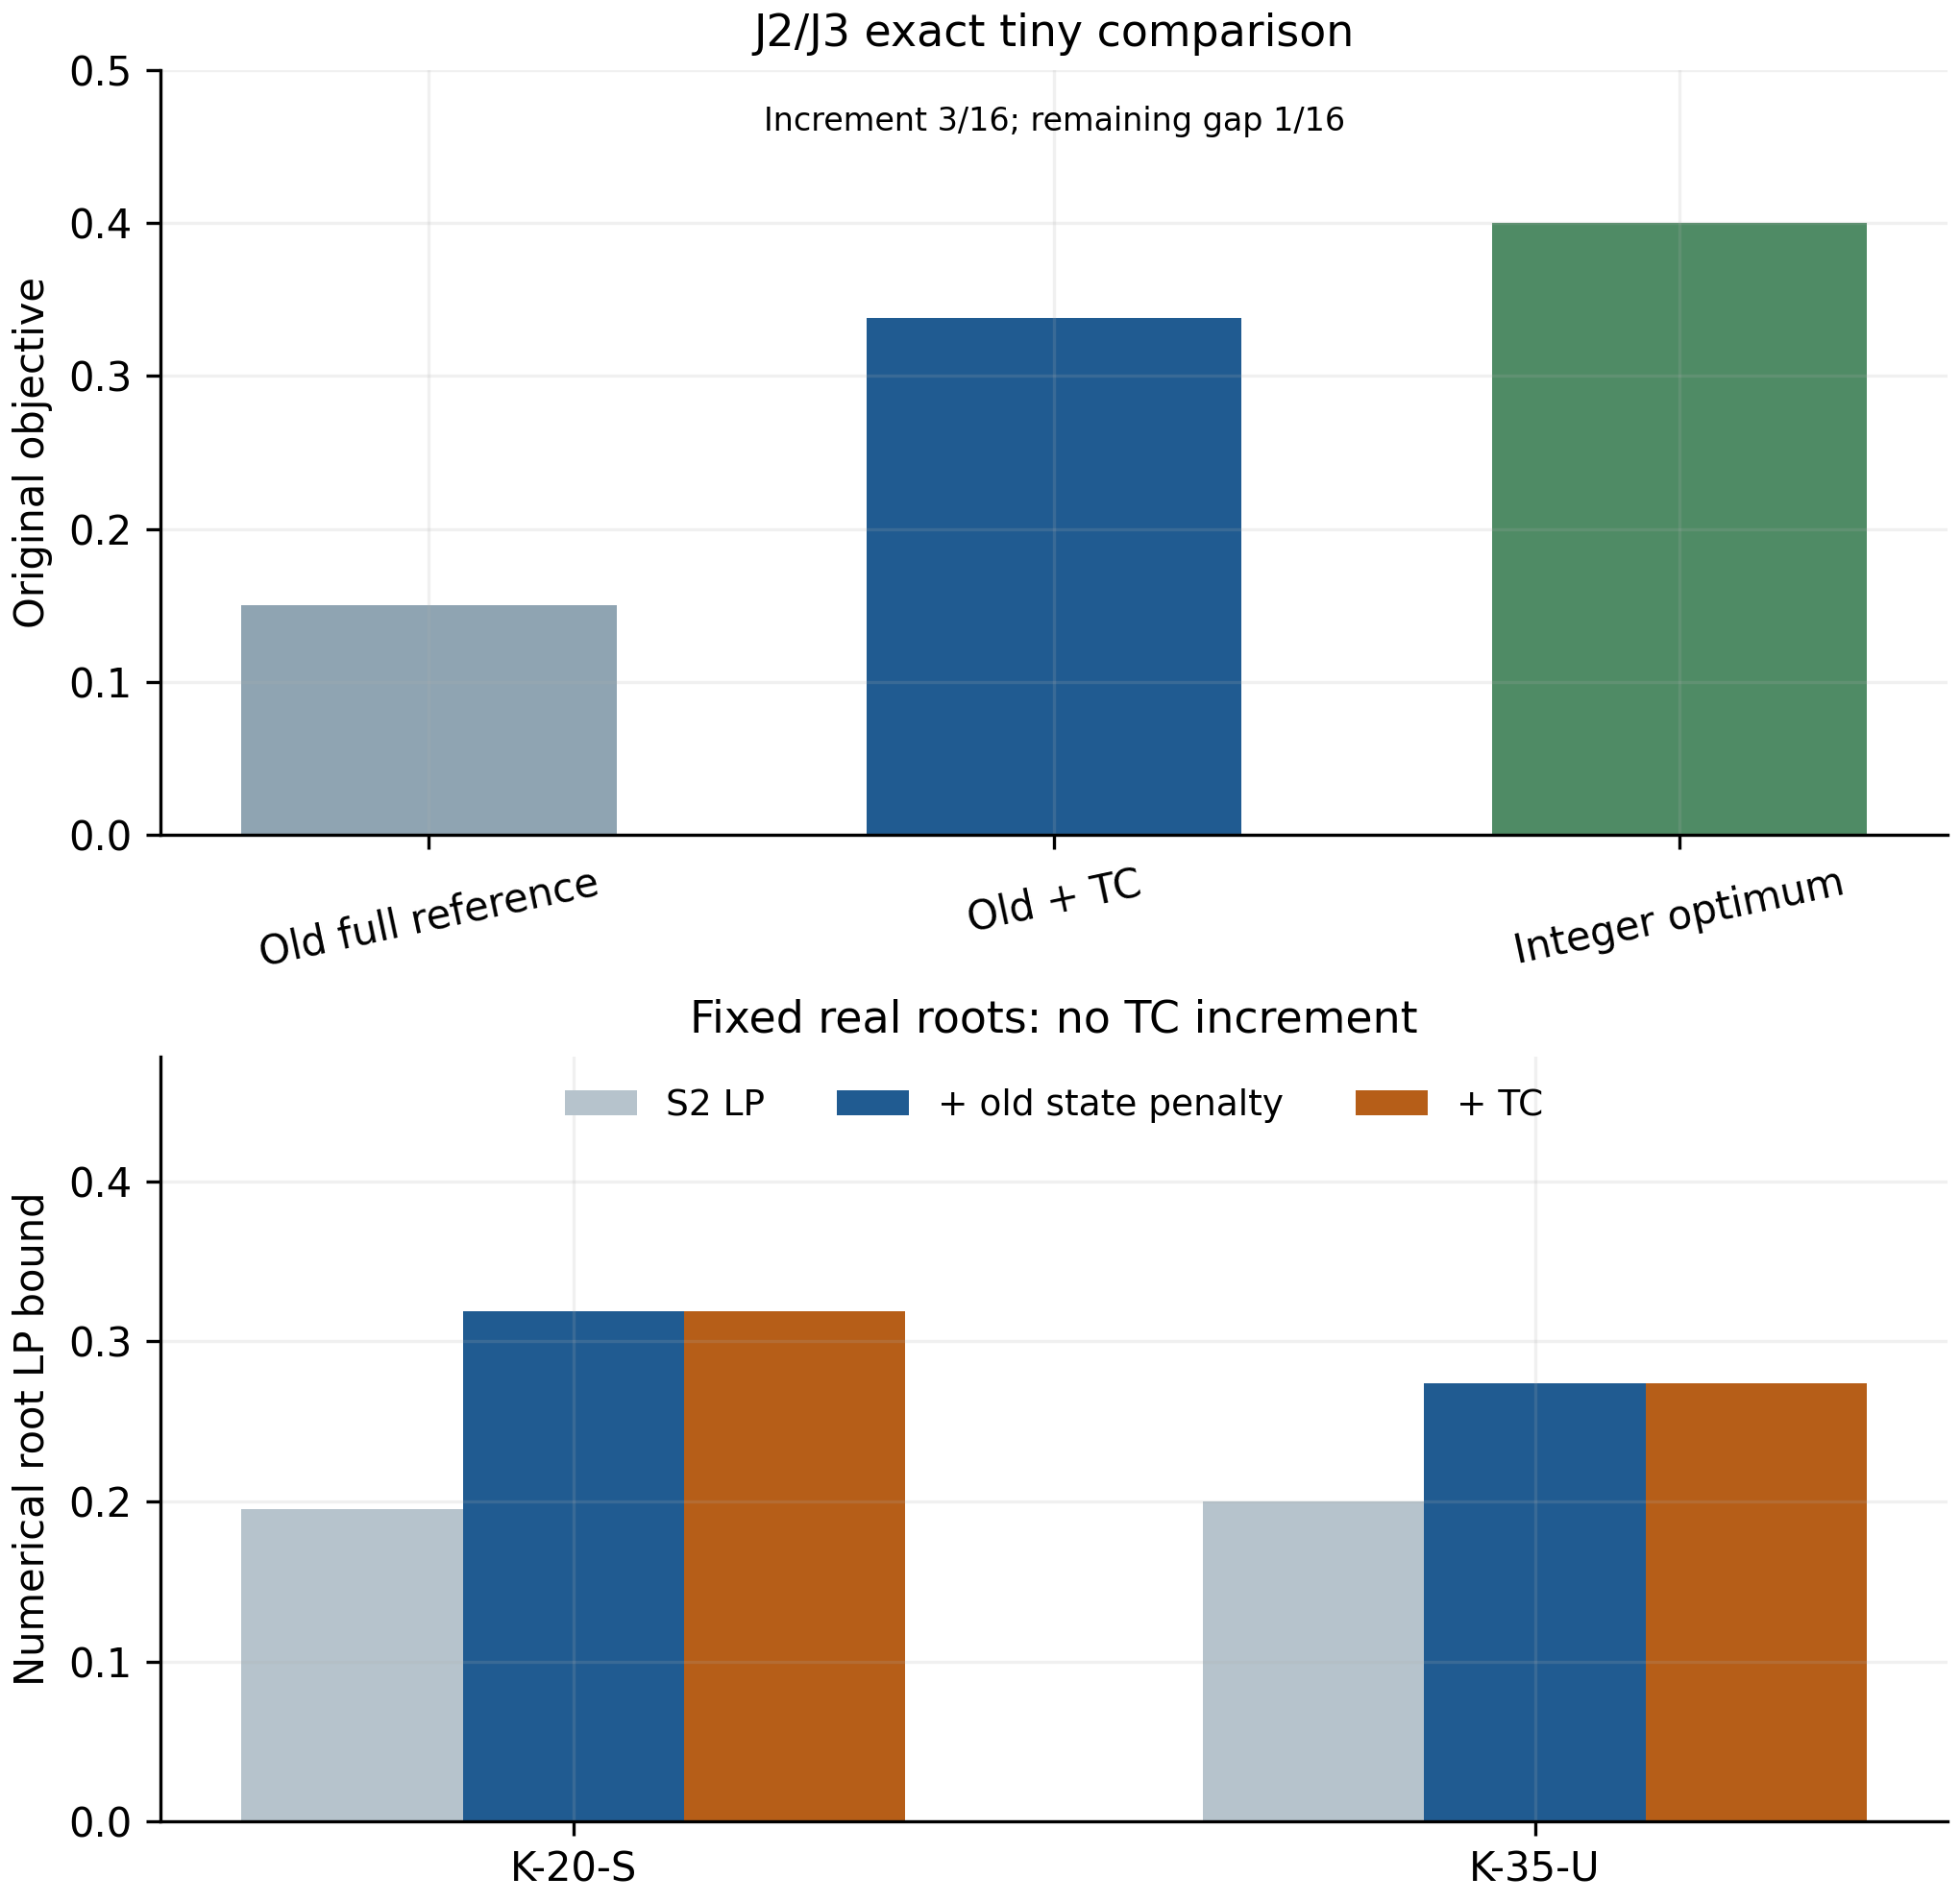
\includegraphics[keepaspectratio,alt={Exact tiny-reference improvement and the separate numerical real-root comparison. Old state penalty is retained before TC is assessed on the real roots.}]{../unified_exact_round135/figures/count_bound_scope.png}}
\caption{Exact tiny-reference improvement and the separate numerical
real-root comparison. Old state penalty is retained before TC is
assessed on the real roots.}
\end{figure}

\paragraph{S8. Source provenance}\label{s8.-source-provenance}

The experimental coordinates/capacities, generated operational fields
and solver outcomes have separate origins. No field is described as
observed demand unless its source actually provides it.

\Needspace{182pt}

{\def\LTcaptype{none} % do not increment counter
\begin{longtable}[]{@{}
  >{\raggedright\arraybackslash}p{(\linewidth - 6\tabcolsep) * \real{0.2500}}
  >{\raggedright\arraybackslash}p{(\linewidth - 6\tabcolsep) * \real{0.2500}}
  >{\raggedright\arraybackslash}p{(\linewidth - 6\tabcolsep) * \real{0.2500}}
  >{\raggedright\arraybackslash}p{(\linewidth - 6\tabcolsep) * \real{0.2500}}@{}}
\toprule\noalign{}
\begin{minipage}[b]{\linewidth}\raggedright
Source
\end{minipage} & \begin{minipage}[b]{\linewidth}\raggedright
Actual archived authority
\end{minipage} & \begin{minipage}[b]{\linewidth}\raggedright
Coordinates and capacities
\end{minipage} & \begin{minipage}[b]{\linewidth}\raggedright
Generated fields and experimental use
\end{minipage} \\
\midrule\noalign{}
\endhead
\bottomrule\noalign{}
\endlastfoot
CITI & R57 source\_\allowbreak{}station\_\allowbreak{}table.csv, SHA256
9f9aad24\allowbreak{}e61d6619\allowbreak{}71c24c6f\allowbreak{}5ec78a69\allowbreak{}081edf01\allowbreak{}ffc43356\allowbreak{}3e52a70b\allowbreak{}2eaca2d0 &
Row-aligned 443-entry local capacity and UTM18N coordinate lists from
the sibling Hybrid GA project; one zero-capacity row remains in the
source but is ineligible for service subsets & K-15-S/K-20-S and earlier
CITI roles; positive targets, initial inventory, weights, centroid
depot, horizons and fleets follow recorded recipes \\
CABI & Official station\_\allowbreak{}information response captured 12 October 2026
05:32:01 UTC, SHA256
d4e664c3\allowbreak{}ecb8c580\allowbreak{}e95d3954\allowbreak{}1555be9c\allowbreak{}f592666a\allowbreak{}515cb854\allowbreak{}a857fb1d\allowbreak{}117ff0b8; 865
station rows & R116 request receipt, row decisions and
source\_\allowbreak{}station\_\allowbreak{}table.csv; EPSG:4326 to EPSG:32618, metre coordinates
rounded to .001 & K-35-U, UC-B20-B, SM-B10-B and other CABI roles;
operating fields are synthetic, not the feed's live availability \\
DIVVY Chicago & Official station\_\allowbreak{}information snapshot captured 23
October 2026 14:54:37 UTC, SHA256
abec7e9a\allowbreak{}784c78b5\allowbreak{}5c1d1f19\allowbreak{}bd4e49fd\allowbreak{}4776f87b\allowbreak{}f9b56fc4\allowbreak{}8b2f2b10\allowbreak{}7b9f2324 & 2,076
raw/2,062 qualified rows; EPSG:4326 to EPSG:32616, .001-metre rounding;
missing/conflicting/virtual records handled by frozen rules & X roles
including X-35-B; same generated inventory/target/weight mechanism on a
third geographic source \\
R55 D13 & Original high\_\allowbreak{}imbalance\_\allowbreak{}seed3201.txt, SHA256
ce60fd4e\allowbreak{}74ad2317\allowbreak{}4be2d4a0\allowbreak{}8ca6e52c\allowbreak{}0043cee2\allowbreak{}2f3c9b17\allowbreak{}153b9e8b\allowbreak{}bcfdbe42 &
Deterministic three-cluster synthetic metric construction, seed 3201 &
Entirely synthetic capacities/inventories/targets/weights; 20 stations,
three Q=30 vehicles, T=3,600 seconds; retained historical adverse-input
role \\
\end{longtable}
}

The CITI capacity and coordinate files have SHA256
92ca9b05\allowbreak{}e66d1425\allowbreak{}bbc801be\allowbreak{}2dd9c077\allowbreak{}6b1a9707\allowbreak{}e62a60b8\allowbreak{}21d941aa\allowbreak{}98625ae1 and
c5fd892c\allowbreak{}c82e0733\allowbreak{}2d4796ed\allowbreak{}b0527182\allowbreak{}d9c60883\allowbreak{}acc9b87a\allowbreak{}5410dab5\allowbreak{}69f990d1. They
contain no station IDs. Canonical identity is the zero-based source row;
companion station names/IDs are annotations and do not re-pair
coordinate/capacity rows. Their original download URL/date and the
provenance of this earlier 443-row selection are not present in the
inspected source record. Those are the specific remaining CITI author
checks; the later CABI and Divvy acquisitions have actual request
receipts.

The CABI original endpoint is
https://gbfs.lyft.com/gbfs/2.3/dca-cabi/en/station\_\allowbreak{}information.json.
Divvy discovery uses https://gbfs.divvybikes.com/gbfs/2.3/gbfs.json and
its recorded station\_\allowbreak{}information member. Source rows require finite
valid coordinates, a unique station ID when the source supplies one,
nonvirtual physical status and integer capacity between 1 and 99.
Identical duplicate records can be coalesced; conflicting duplicates are
excluded. Snapshots and row decisions fix the actual results
independently of later live-feed changes.

Selections use frozen hash-derived seeds, source-row tie breaking,
compact nearest-station or regional farthest-first rules, and recorded
exposure exclusions. A per-input selection record lists every source
row. The landscape record links its source hash and selection to
positive synthetic targets, initial stocks and generated weights.
Targets follow the recorded capacity-fill rule; shortage/balance/surplus
totals and local adjustments follow deterministic recipes. Current
generated weights are max(0.1,(D\_\allowbreak{}i/max\_\allowbreak{}j D\_\allowbreak{}j)\^{}2), rounded to six
decimals, with maximum 1; they are not sum-normalized. The legacy D13
weight construction retains its original file rather than adopting this
later rule.

Depots are artificial centroids with parser compatibility placeholders.
The fleet starts empty regardless of the depot's placeholder inventory.
Serialized planar metre coordinates determine Euclidean travel time at
1.5 m/s; per-unit pickup/drop handling is 60 seconds. Horizons and
fleets are experiment design parameters. The min\_\allowbreak{}ratio field is
compatibility metadata, not a service-floor constraint. No trip history
or dynamic demand is used.

Public source material is attributed through the providers' system-data
and license links and is used within the noncommercial research study.
This round adds no standalone provider dataset and redistributes no
private author manuscript. Published input derivatives and previously
archived sources retain their fixed-commit records.

Machine-readable source and input hashes for the seven registered R135
roles are in the
\href{https://github.com/yifanXovo/TailoredExact/blob/codex/round166-structure-and-paper/results/unified_exact_round135/input_provenance.json}{historical
input provenance}. Full historical source metadata remains pinned to the
recorded R57/R116/R132 commits; no complete old campaign is restored.

\paragraph{S9. Source access and specific literature
differences}\label{s9.-source-access-and-specific-literature-differences}

The model and decoder descend from the available HGA-TGBC author draft,
\emph{Equity-aware Bike Repositioning in Station-based Bike-sharing
Systems}. The locally available May 2026 file was rechecked and matches
the earlier inspected identity; it is not asserted to be the latest
version. Private text is not redistributed. The bibliography attributes
the actual available draft.

The targeted
\href{https://github.com/yifanXovo/TailoredExact/blob/codex/round166-structure-and-paper/results/unified_exact_round165/literature_review.md}{primary-source
review} records the formal Gupte §2.1 read, Köppe's author-version §2
read, inherited BRP model comparisons and access boundaries.
McCormick/convexity tools remain standard background. The paper's
single-product projection and state-penalty arguments are proved
directly.

Qiao et al.'s publisher-indexed abstract/highlights describe
task-duration fairness and coordinated inter-/intra-zone echelons.
Caggiani et al.'s official institutional abstract describes
availability/state-of-charge Gini, zonal targets, relocation and battery
swapping with microsimulation. These read locations support the
different equity objects stated in §1.1. Complete formulation relations
are unknown: no equivalence, strict separation, dominance or priority
claim is inferred. The openly listed Caggiani VoR could not be read: web
content-size failure and one normal direct-download HTTP403 are recorded
without a paywall diagnosis or configuration change.

The original CITI capture URL/date and station IDs remain unavailable.
Archived row identity, coordinates/capacity and frozen selection bind
the inputs; CABI/Divvy have their actual acquisition receipts. Current
live feeds are provider references, not replacements for historical
snapshots.

\paragraph{S10. Historical evidence and finite
reproduction}\label{s10.-historical-evidence-and-finite-reproduction}

R132 breadth retains 17/24 S2, 9/24 P and 4/12 PS qualified certificates
under its original policy. R133 retains fourteen exposed qualification
positions and its four-pair old/new bridge. R134 retains S2 12/14, P
9/14 and PS 2/4 across 32 method positions. These layers are neither
pooled as independent input samples nor relabelled by later source
policies. Full older tables remain at their fixed commits, including the
\href{https://github.com/yifanXovo/TailoredExact/tree/29adc14cf2089442298b409ba2bc06963e77bc14/results/unified_exact_round134}{R134
scientific evidence}, and the R132/R133 citations recorded there.

Current reproduction replays all entered R135 positions and the two AP
root coefficient/residual records from exact source-byte and raw
carriers. It invokes no Optimize, compiler or vendor DLL. Historical
whole campaigns and unentered conditional positions are not
reconstructed. Source/PE/DLL/input identity, all ordinary outcomes,
failed attempts and measured costs remain separate from the authorship
and journal-format checks required before actual submission.

\paragraph{S11. Maintained historical controls and equivalent-expression
proofs}\label{s11.-maintained-historical-controls-and-equivalent-expression-proofs}

MD-R version 1 is a research ablation, not another proposed algorithm.
Historical supplement
\href{https://github.com/yifanXovo/TailoredExact/blob/39043b15b3cceae2cab14a3fbaec39e2b16339ce/results/unified_exact_round130/manuscript.md}{the
R130 historical account} Section 6.8 and the root contract define its
same-H inclusive domain, semantic shortcut omission, mandatory actual
own-Start pre-LP check, one LP plus one integer MIP, fixed cutoff and
complete native optimal-root return obligation. It retains the physical
and signed numerical evidence policy. TIME\_\allowbreak{}LIMIT/INTERRUPTED may yield
a qualified open endpoint with null T\_\allowbreak{}cert; a near-equal bound alone
cannot satisfy its missing optimal-return obligation. Its extra checks
and complete costs are paid. These control-specific guards leave the
frozen ordinary procedure and the historical evidence in this appendix
unchanged.

\subparagraph{B.13 Uniform support candidate confirmation
(Round129)}\label{b.13-uniform-support-candidate-confirmation-round129}

Round129 changes no production source, H, model generator, numerical
policy or controller. It reuses original E2 modes mb/ms2/p.~The sole
candidate MS2 suppresses triple support for every input while retaining
pairs, ordered supply and the shared enumeration order/cap. The five
fixed candidate rules and thirty complete paid observations are in
\href{https://github.com/yifanXovo/TailoredExact/blob/39043b15b3cceae2cab14a3fbaec39e2b16339ce/results/unified_exact_round130/manuscript.md}{the
R130 historical account} Section 6.9. At the R129 selection stage, MS2
was the proposed candidate and full M-B was the then-current frozen
method. That historical distinction and all tables remain; R130 adopted
S2/MS2 as the sole paper method, unchanged through Round132. The
independent finite review and public recovery are evidence checks, not
new native solves or rational proofs of all matrices.

\subparagraph{B.14 Historical pair-support adoption and attribution
controls}\label{b.14-historical-pair-support-adoption-and-attribution-controls}

The sole paper method retains the historical E2
\texttt{ms2} identity, called S2. Historical E3 retains
that version's source behavior and adds the off-by-default unique
\texttt{s2-\allowbreak{}root} identity plus PS parameter evidence
readback. E2 is retained unchanged. PS reuses the full original-compact
mapper/validator; S2R reuses R128 inclusive-root semantics with triple
emission disabled. Historical supplement
\href{https://github.com/yifanXovo/TailoredExact/blob/39043b15b3cceae2cab14a3fbaec39e2b16339ce/results/unified_exact_round130/manuscript.md}{the
R130 historical account} Section 6.10 states the paid workflows, exact
cutoff complement, nonzero LP/MIP obligations, source/return/coverage
requirements, actual exposure and attribution limits. No individual cut,
H, threshold or native parameter is optimized here. The passed R129
candidate selection is not rerun.

\clearpage

\subparagraph{Appendix C. Equivalent-expression proofs and actual-model
conditions}\label{appendix-c.-equivalent-expression-proofs-and-actual-model-conditions}

\subparagraph{C.3. Projection of the three geometry row
families}\label{c.3.-projection-of-the-three-geometry-row-families}

Delete only H-spread, variable-\(S\) centering and fixed-\(S\)
centering. Keep all \(H\) absolute-value lower bounds, individual
bounds, total cap/floor, original Gini epigraph, scalar/SP estimators,
cutoff, real domains and domain-generation rules. For \(n\ge2\) the
ideal three families are

\[
(n-1)H_{ij}\le n\beta S,\quad
\pm(n-1)(r_i-r_j)\le n\beta S,\quad
\pm(r_i-r_j)\le \frac{n\beta\bar S}{n-1}.
\]

Let \(H_\Sigma=\sum_{i<j}H_{ij}\). The retained original epigraph is
\(H_\Sigma\le n\sum_i Z_i/D_i\). Nonnegative states and
\(q_{iy}\le\beta s_{iy}\) give \(Z_i\le\beta Y_i\), hence
\(H_\Sigma\le n\beta S\). Triangle inequalities give
\(A\ge(n-1)|r_i-r_j|\): for each third station \(t\),
\(|r_i-r_t|+|r_t-r_j|\ge|r_i-r_j|\), together with the pair itself;
unused pair distances are nonnegative. Thus both centering families
follow from the retained inequalities and \(S\le\bar S\).

\subparagraph{Root interval}\label{root-interval}

When \(\alpha=0\), replace every \(H_{ij}\) by \(|r_i-r_j|\). This
decreases the sum, respects its upper bounds and all individual upper
bounds under the audited conditions, and the floor reduces to
nonnegativity. The new \(H\) satisfies H-spread and leaves all non-\(H\)
variables and the objective unchanged. Reverse inclusion follows by
adding constraints. Thus projecting away all \(H\) gives equal LP sets
and equal ideal LP objective values. Because \(H\) is continuous, the
same extension preserves any remaining integer restrictions.

\subparagraph{Positive lower endpoint}\label{positive-lower-endpoint}

Assume \(0\le\alpha\le\beta\), \(r_i\ge0\), \(S\le\bar S\); individual
\(H\) upper bounds \(U_{ij}=c_i+c_j\) with \(c_i\ge0\) and
\(r_i\le c_i\); and outside the deleted families \(H\) appears only in
absolute lower bounds, individual bounds, a total floor/cap and other
uniform total upper bounds. It has zero objective coefficient and no
additional individual positive lower bounds or nonuniform linear uses.

Fix every non-\(H\) variable in a feasible point of the deletion model.
Put \(d_{ij}=|r_i-r_j|\), \(A=\sum_{i<j}d_{ij}\), \(L=n\alpha S\) and
\(t=n\beta S/(n-1)\). Let \(B\) be the smallest retained total upper
bound, including the implied \(n\beta S\). Feasibility gives

\[
T^*=\max(A,L)\le\min\left(B,\sum_{i<j}U_{ij}\right).
\]

The triangle argument gives \(d_{ij}\le t\). Set
\(U'_{ij}=\min(c_i+c_j,t)\). For \(C=\sum_i c_i>0\), the function
\(f(\mathbf c)=\sum_{i<j}\min(c_i+c_j,t)\) is concave on the nonnegative
simplex of sum \(C\). With \(e_i^{\rm unit}\) denoting the standard unit
vector, write \(\mathbf c=\sum_i(c_i/C)C e_i^{\rm unit}\). Concavity
gives

\[
\sum_{i<j}U'_{ij}=f(\mathbf c)\ge(n-1)\min(C,t)
=\min\left(\sum_{i<j}U_{ij},n\beta S\right)\ge T^*.
\]

If \(\sum_{i<j}U'_{ij}>A\), set

\[
\theta=\frac{T^*-A}{\sum_{i<j}U'_{ij}-A},\qquad
H'_{ij}=d_{ij}+\theta(U'_{ij}-d_{ij}).
\]

Then \(0\le\theta\le1\); every individual bound and spread bound holds,
\(\sum_{i<j}H'_{ij}=T^*\le B\), and the floor holds. The centering rows
already follow without \(H\). All non-\(H\) variables and their
objective remain unchanged. If the denominator vanishes, \(T^*=A\) and
\(H'=d\) suffices. If \(C=0\), all \(c,r,S,A,L\) vanish and \(H'=0\). If
\(S=0\), nonnegative ratios vanish and \(H'=0\). For \(n=1\) none of
these three families is generated. This proves both projected
inclusions, including the nonzero-floor case in which setting \(H=d\)
alone can fail.

\subparagraph{Actual-model application and numerical
boundary}\label{actual-model-application-and-numerical-boundary}

The current shared canonical factory generates the named three families,
and the frozen paper profile disables local/subset nonuniform \(H\)
uses. The Cplex writer sets \(H\) upper bounds to
\(\operatorname{fl}(C_i/D_i+C_j/D_j)\), with zero objective
coefficients. The independent reviewer inspected an actual saved S12 S2R
matrix: 66 \(H\) bounds, five uniform full-\(H\) rows and 198
individual-\(H\) rows. \(W\) appears in five rows, as required below.
This is a canonical-model result, not a theorem about arbitrary native
node cuts.

The exact additive upper-bound hypothesis concerns real algebra. In the
saved S12 matrix, 41 of 66 serialized \(H\) bounds differ from the exact
rational sum of the two serialized \(r\) upper bounds at roughly
\(10^{-16}\). Therefore the ideal theorem is not asserted as strict
rational equality for every serialized floating matrix. Necessary actual
coefficient/domain checks and extension residuals accompany the research
comparisons. In that frozen R132 expression study the production S2
bytes were unchanged and no hidden outward correction was applied. The
later candidate's explicit inclusive-cutoff repair has a separate
identity and is not attributed to expression deletion. Equal projections
do not imply identical presolve, native cuts, search paths or elapsed
time, and do not make the entire \(C_G\) package redundant.

\subparagraph{C.4. Exact elimination of W, including its real
bounds}\label{c.4.-exact-elimination-of-w-including-its-real-bounds}

In the active shared model \(W=W_{\rm SP}\) is continuous, has zero
objective coefficient and is used by four MC rows, one SP cutoff and its
own box. No other use is present in the qualified canonical scope.
Preserve all \(W\)-free original rows, variable types and bounds,
particularly \(g+\lambda P\le c\), which a cross-multiplied row cannot
replace at \(S=0\).

For actual \(W\) bounds \(w_l,w_u\) and MC parameters
\(s_l,s_u,p_l,p_u\), define

\[
L_0=w_l,\quad L_1=s_lP+p_lS-s_lp_l,\quad
L_2=s_uP+p_uS-s_up_u,
\] \[
U_0=w_u,\quad U_1=s_uP+p_lS-s_up_l,\quad
U_2=s_lP+p_uS-s_lp_u.
\]

The original system is \(L_j\le W\le U_k\) and
\(H_\Sigma+n\lambda W\le ncS\). For \(\lambda>0\), its complete
projection is all nine compatibility rows \(L_j\le U_k\) and all three
lower-cutoff rows \(H_\Sigma+n\lambda L_j\le ncS\). Necessity is
immediate. Conversely, \(W=\max_jL_j\) satisfies every upper bound and
the SP cutoff, proving sufficiency. This is standard one-variable
Fourier-Motzkin elimination applied to this formulation, not a new
linearization theorem or an exact continuous product identity.

Only after proving the same explicit nonnegative rectangle
\(0\le s_l\le S\le s_u\), \(0\le p_l\le P\le p_u\), and that the actual
\(W\) box is no tighter than the product box, may compatibility and box
rows be removed. The true product \(SP\) is then an extension for MC
feasibility. Since \(L_1-s_lp_l=s_l(P-p_l)+p_l(S-s_l)\ge0\) and
\(w_l\le s_lp_l\), the constant lower plane is dominated. The two
lower-plane cutoffs then suffice, with \(W=\max(L_1,L_2)\). Current
inflated \(e\) can violate the tight physical \(P\) upper estimate; that
estimate cannot simply be assumed to bound the whole epigraph.

For positive width \(s_u>s_l\), MC lower/upper pairings imply
\(P\ge p_l\) and \(P\le p_u\) after cancellation. These consequences
must survive projection. For example,
\(s_l=1,s_u=2,p_l=0,p_u=1,S=1,P=2,H_\Sigma=0\) and sufficiently large
\(c\) satisfy both lower-plane cutoffs, but \(L_2=3>U_2=2\), so no
original \(W\) exists. Two cutoffs alone would incorrectly enlarge the
domain.

When \(S\) is fixed, derive compatibility directly rather than dividing
by its width. At \(S=0\), \(W=0\) need not imply \(P\le p_u\). The full
pair system handles that case without adding an unauthorized \(P\)
bound. When \(\lambda=0\), retain \(H_\Sigma\le ncS\) and every
\(W\)-feasibility compatibility row; removing the whole block would
again change its projection. Zero-width \(P\) and simultaneous
degeneracy are also covered by the pair construction.

\subparagraph{Implemented research
expression}\label{implemented-research-expression}

The research writer reads the actual shared canonical row coefficients,
normalizes their senses, includes the exact actual \(W\) box, and
combines every lower/upper pair. There are three lower rows and four
upper rows including the SP row: 12 projected rows. It retains even
constant or duplicate compatibility rows. All remaining original rows,
objective, bounds and integer types stay intact; only the \(W\) column
and its rows are replaced. Its physical Start is mapped to the remaining
actual columns and validated before use.

The independent checker reconstructs these combinations with exact
rational arithmetic on source binary64 coefficients. It separately
bounds the output coefficient-serialization residual over actual
remaining-variable bounds. The candidate binary64 output is qualified as
numerically consistent, not asserted to equal the exact rational
projected matrix.
\texttt{C\_\allowbreak{}matrix\_\allowbreak{}wording\_\allowbreak{}addendum.json} makes this
distinction explicit. Four saved interval/input configurations have
equal canonical all-continuous LP objectives within the inherited
\(10^{-7}\) policy. These finite observations check implementation and
numerical behavior; they do not replace the general projection proof.

\subparagraph{C.5. Qualification and relation to
costs}\label{c.5.-qualification-and-relation-to-costs}

The research default-off writer and original E3 produce identical
complete canonical LP bytes on the qualified small and medium fixtures,
at a root interval and a positive lower endpoint. Actual S12 CLI runs
bridge original E3 to research default-off, and validate independent H
and full Start submission for both candidates. Each uses the legal
inclusive-root LP then restored-integer MIP workflow. Default-off
equivalence is a semantic/matrix bridge; the two executable byte strings
are different and are never described as identical.

All 24 admitted C workflows are now sealed. Geometry deletion gives 2
Win, 4 Lose and 2 UNDETERMINED; full W projection gives 3 Win, 3 Lose
and 2 UNDETERMINED against the same-build inclusive-root baseline. All
16 candidate/baseline comparisons have identical complete realized H,
matching root intervals/cutoffs and actual native exposure. The
continuous root objectives agree within the original numerical policy,
while Work/nodes and complete costs vary in both directions. This
supports mixed expression costs, not a stronger ideal relaxation or
automatic production replacement. D remains the original frozen
algorithm and its measurements do not come from this research build.

\subsection{Round163 structural-stage evidence and prospective
protocol}\label{round163-structural-stage-evidence-and-prospective-protocol}

The original R132/R134/R137 observations above retain their measured
versions, Seeds, budgets and denominators. They are not concatenated
with Round163 as independent samples. The frozen B/E+/P comparison has
six new configurations, 18 separately paid arms, one Gurobi Seed and no
result-dependent redraw or candidate switch. It is prospective
confirmation on archived-source station data with synthetic
inventories/targets/weights, not new cities or independent
observed-demand validation. All six become exposed after this study.

The
\href{https://github.com/yifanXovo/TailoredExact/blob/codex/round166-structure-and-paper/results/unified_exact_round163/source_recipe.json}{fixed
recipe},
\href{https://github.com/yifanXovo/TailoredExact/blob/codex/round166-structure-and-paper/results/unified_exact_round163/input_manifest.json}{six-input
identities},
\href{https://github.com/yifanXovo/TailoredExact/blob/codex/round166-structure-and-paper/results/unified_exact_round163/source_overlap.json}{source
overlap disclosure} and
\href{https://github.com/yifanXovo/TailoredExact/blob/codex/round166-structure-and-paper/results/unified_exact_round163/matrix_frozen.json}{18
complete commands} preserve the pre-performance protocol. The
\href{https://github.com/yifanXovo/TailoredExact/blob/codex/round166-structure-and-paper/results/unified_exact_round163/structural_synthesis.md}{stage
synthesis} gives the
inherited-conclusion/evidence/new-increment/inference-boundary table;
its
\href{https://github.com/yifanXovo/TailoredExact/blob/codex/round166-structure-and-paper/results/unified_exact_round163/historical_source_map.json}{source
map} binds all 25 directly read files to fixed commits and byte hashes.
The expanded
\href{https://github.com/yifanXovo/TailoredExact/blob/codex/round166-structure-and-paper/results/unified_exact_round137/mathematical_analysis.md}{mathematical
analysis} states the actual helper epigraph objective, nested-domain
premises, coverage/cutoff contracts and gap identity. No previous
producer or full historical raw carrier is replayed.

The three methods share the actually hashed R162 complete\_\allowbreak{}v2 C++
executable and Gurobi 13.0.2. E+ additionally invokes the unchanged
historical Python RN16384 inventory helper on its own canonical root;
its mixed implementation and complete paid cost are explicit. Every arm
has one production deadline. The ordinary C++ methods, helper, stable
profiles, complete physical objective, loaded-return convention and
numerical qualification remain fixed. The final tables and algorithm
choice are appended only after all 18 arms and their original-objective
audits close.

\subsection{Round163 completed configuration
evidence}\label{round163-completed-configuration-evidence}

All six first-valid inputs and all 18 qualified endpoints are retained.
The
\href{https://github.com/yifanXovo/TailoredExact/blob/codex/round166-structure-and-paper/results/unified_exact_round163/reports/complete.csv}{complete
table},
\href{https://github.com/yifanXovo/TailoredExact/blob/codex/round166-structure-and-paper/results/unified_exact_round163/reports/complete_arms.json}{binary64
endpoints},
\href{https://github.com/yifanXovo/TailoredExact/blob/codex/round166-structure-and-paper/results/unified_exact_round163/reports/comparisons.csv}{three
comparisons} and
\href{https://github.com/yifanXovo/TailoredExact/blob/codex/round166-structure-and-paper/results/unified_exact_round163/final_report.md}{helper/fee
interpretation} give the full denominator, original gap policy,
T\_\allowbreak{}cert/T\_\allowbreak{}produce/T\_\allowbreak{}verify/T\_\allowbreak{}total, actual Native Work/nodes, own-H
and helper costs.
\href{https://github.com/yifanXovo/TailoredExact/blob/codex/round166-structure-and-paper/results/unified_exact_round163/decision.json}{Stage
choice},
\href{https://github.com/yifanXovo/TailoredExact/blob/codex/round166-structure-and-paper/results/unified_exact_round163/cost_report.json}{closed
fees} and
\href{https://github.com/yifanXovo/TailoredExact/blob/codex/round166-structure-and-paper/results/unified_exact_round163/science_identity.json}{science
identities} separate the paper algorithm, frozen research implementation
and released main.

Retain uniform GI-TBC/B as the paper's main algorithm. Keep uniform E+
as a separately named, limited proof enhancement, with its genuine X35
gain and earlier qualified R154/R156 gains preserved. This complete
panel does not justify replacing B as the main recommendation; the
current broad-promotion attempt ends here. No per-input best-of-B/E+
method or released-default change is made.

Both B and E+ certify 3/6 configurations, versus cold P 1/6. B/E+ have
identical verified physical U on all six. E+ raises X35's final
qualified L from B's .3949882559151472 to .42319954961578576 at
U=.45747531701601785; the original relative gap falls from
13.659110945800548\% to 7.492375244155952\%. The other five final proof
endpoints are equal. E+'s X35 raw search L is .39492875817006656,
slightly below B's; the improvement is the separate qualified proof
source, not an improved raw AM/Native bound. No additional certificate
or primal improvement is observed.

The three both-certified E+/B paid T\_\allowbreak{}cert ratios are 1.130665945756784,
1.3357446355323432 and 1.0515856109492556. The absolute increases are
about 26.10 s, 1.70 s and 6.18 s on C20, B20 and X20. Only C20 meets the
existing substantive scale max(10 s, 10\% of the faster time); the two
other numerical directions remain recorded as nonmaterial. E+ pays
256.7365551 helper seconds inside the original deadlines. Aggregate
audit-inclusive T\_\allowbreak{}total is 7506.416129835416 s for E+ and
7451.303745185491 s for B, a 55.112384649924934 s increase; helper time
is already included. The genuine X35 proof gain and all equal physical
upper endpoints make uniform E+ a reasonable alternative when proof
information is prioritized. The paper's choice of B balances certificate
count, paid time and both endpoints; it is not a dominance theorem or a
requirement that every input improve.

B and E+ each have lower U than P on three configurations, higher U on
C35-U, and equal U on two. Each has substantively higher proof L than P
on five configurations and equal qualified endpoints on the remaining
certified B20 case. On C35-U, P's U=.09331934374779818 is strictly
better than B/E+'s .12956638965196035, while B/E+ have stronger L; this
opposition is retained. The one joint-CERT B/P or E+/P time ratio
conditions on B20 alone. No full-panel time superiority or universal
P-GRB dominance is inferred from a single Seed.

C20, B20 and X20 finish with search L beyond their qualified inventory
value uppers. C35's inventory result is numerically near zero, not an
exact-zero physical proof. B35 and X35 prices stop at RN16384 with
widths .014387103336740467 and .02295563610060769. B35's returned floor
is below final search L but its inventory upper is above it; X35's floor
contributes to the final proof while its price remains unresolved. Old
R156's small same-domain remainder therefore cannot be generalized to
these new prices. No larger capacity, alternate price, Seed or candidate
is tried.

The
\href{https://github.com/yifanXovo/TailoredExact/blob/codex/round166-structure-and-paper/results/unified_exact_round163/main_table_update.json}{master-table
receipt} appends only verified B/P pairs to the existing CSV copies; E+
is separately labelled throughout. The
\href{https://github.com/yifanXovo/TailoredExact/blob/codex/round166-structure-and-paper/results/unified_exact_round163/final_report.md}{final
report} and
\href{https://github.com/yifanXovo/TailoredExact/blob/codex/round166-structure-and-paper/results/unified_exact_round163/RESUME.md}{delivery/recovery
status} link independent review identities and the bounded new-only
public recovery. Original source-row overlaps and retrospective
master-table reconciliation are disclosed without changing the frozen
generation or selecting on outcomes.

Maintained body, appendices, mathematical companion, bibliography and
figures are the current sources. The manuscript and supplement PDFs are
regenerated by the current component-only build; the Git history retains
the earlier snapshots.

\subsection{Research navigation for saved C35
skeletons}\label{research-navigation-for-saved-c35-skeletons}

The former main-body §7.1 diagnostic work list is retained in
\href{https://github.com/yifanXovo/TailoredExact/blob/codex/round166-structure-and-paper/results/unified_exact_round164/research_navigation.md}{research
navigation}. It reconciles the existing complete R96
fixed-ownership/relative-order quantity object, parent containment and
full physical/epigraph qualifications. No such restricted model, route
oracle, feedback candidate or new producer is executed in the
solver-Seed confirmation. The known feasible P target, an
unserved-station penalty floor and an inventory-only target vector do
not by themselves determine the complete saved-skeleton optimum.
R62/R96/R97/R160 retain their original positive, mixed and adverse
evidence.

\subsection{Round164 completed finite solver-Seed
evidence}\label{round164-completed-finite-solver-seed-evidence}

All 24 registered new B/P positions complete at Seeds1/2, keyed on
input, Seed, method and actual repeat1. Twelve new pairs and six
qualified historical Seed0 pairs form six within-input groups. The
\href{https://github.com/yifanXovo/TailoredExact/blob/codex/round166-structure-and-paper/results/unified_exact_round164/reports/seed_evidence.md}{complete
full-precision evidence tables} report all 36 own-run physical U,
raw/qualified search L, final proof L, original gaps, certificate
states, paid clocks, own-H and Native effort. The
\href{https://github.com/yifanXovo/TailoredExact/blob/codex/round166-structure-and-paper/results/unified_exact_round164/reports/complete.csv}{new
24-arm CSV},
\href{https://github.com/yifanXovo/TailoredExact/blob/codex/round166-structure-and-paper/results/unified_exact_round164/reports/three_seed_comparisons.json}{paired
differences},
\href{https://github.com/yifanXovo/TailoredExact/blob/codex/round166-structure-and-paper/results/unified_exact_round164/reports/within_configuration.json}{within-input
summaries} and
\href{https://github.com/yifanXovo/TailoredExact/blob/codex/round166-structure-and-paper/results/unified_exact_round164/final_report.md}{finite
report} retain every OPEN observation and both endpoint directions. No
E+ floor is included in B.

Historical Seed0 reuses the same input/physical/method/PE/DLL/deadline
and numerical contracts. Its selected original physical fleets and all
Native Seed settings are reread; live OS module/affinity records and
original native CPU/Windows/Gurobi headers match both new Seeds. The
\href{https://github.com/yifanXovo/TailoredExact/blob/codex/round166-structure-and-paper/results/unified_exact_round164/Seed0_reuse_qualification.json}{reuse
qualification} does not assert identical incidental OS load or
statistical exchangeability. The
\href{https://github.com/yifanXovo/TailoredExact/blob/codex/round166-structure-and-paper/results/unified_exact_round164/science_identity.json}{identity
audit} binds all 24 fresh serial lifecycles and independently paid
fixed-seed H.

\subsubsection{Descriptive within-input
summaries}\label{descriptive-within-input-summaries}

The medians and ranges below summarize three differences, not a new
feasible solution, proof endpoint or independent sample. Full binary64
values and tolerance-qualified signs remain in the linked machine
reports.

\Needspace{226pt}

{\def\LTcaptype{none} % do not increment counter
\begin{longtable}[]{@{}
  >{\raggedright\arraybackslash}p{(\linewidth - 4\tabcolsep) * \real{0.3333}}
  >{\raggedright\arraybackslash}p{(\linewidth - 4\tabcolsep) * \real{0.3333}}
  >{\raggedright\arraybackslash}p{(\linewidth - 4\tabcolsep) * \real{0.3333}}@{}}
\toprule\noalign{}
\begin{minipage}[b]{\linewidth}\raggedright
Input
\end{minipage} & \begin{minipage}[b]{\linewidth}\raggedright
Median ΔU {[}minimum, maximum{]}
\end{minipage} & \begin{minipage}[b]{\linewidth}\raggedright
Median ΔL {[}minimum, maximum{]}
\end{minipage} \\
\midrule\noalign{}
\endhead
\bottomrule\noalign{}
\endlastfoot
R163-C20-S & 0 {[}-0.05927393, 0{]} & 0.03369846 {[}0.03104638,
0.03941158{]} \\
R163-B20-B & 0 {[}0, 0{]} & 3.885781e-16 {[}5.551115e-17,
2.090347e-10{]} \\
R163-X20-S & -0.01320014 {[}-0.01721348, -0.01320014{]} & 0.1948245
{[}0.186098, 0.1974955{]} \\
R163-C35-U & -0.03868052 {[}-0.05019445, 0.03624705{]} & 0.01155073
{[}0.009334378, 0.01347433{]} \\
R163-B35-S & -0.101716 {[}-0.13296, -0.0549627{]} & 0.004752414
{[}0.004661458, 0.006254594{]} \\
R163-X35-S & -0.06178785 {[}-0.08405536, -0.06065283{]} & 0.04442013
{[}0.03201682, 0.04660159{]} \\
\end{longtable}
}

\subsubsection{Joint-CERT paid time
intersection}\label{joint-cert-paid-time-intersection}

The intersection is exactly B20, 1/6 inputs at each Seed (three
within-input pairs overall). Every listed difference exceeds its 10 s
substantive scale. OPEN observations supply no convergence time and are
not removed to infer a full-panel acceleration.

\Needspace{160pt}

{\def\LTcaptype{none} % do not increment counter
\begin{longtable}[]{@{}
  >{\raggedright\arraybackslash}p{(\linewidth - 10\tabcolsep) * \real{0.1667}}
  >{\raggedright\arraybackslash}p{(\linewidth - 10\tabcolsep) * \real{0.1667}}
  >{\raggedright\arraybackslash}p{(\linewidth - 10\tabcolsep) * \real{0.1667}}
  >{\raggedright\arraybackslash}p{(\linewidth - 10\tabcolsep) * \real{0.1667}}
  >{\raggedright\arraybackslash}p{(\linewidth - 10\tabcolsep) * \real{0.1667}}
  >{\raggedright\arraybackslash}p{(\linewidth - 10\tabcolsep) * \real{0.1667}}@{}}
\toprule\noalign{}
\begin{minipage}[b]{\linewidth}\raggedright
Seed
\end{minipage} & \begin{minipage}[b]{\linewidth}\raggedright
B20 B T\_\allowbreak{}cert
\end{minipage} & \begin{minipage}[b]{\linewidth}\raggedright
B20 P T\_\allowbreak{}cert
\end{minipage} & \begin{minipage}[b]{\linewidth}\raggedright
ΔT=B−P /s
\end{minipage} & \begin{minipage}[b]{\linewidth}\raggedright
B/P
\end{minipage} & \begin{minipage}[b]{\linewidth}\raggedright
Substantive scale /s
\end{minipage} \\
\midrule\noalign{}
\endhead
\bottomrule\noalign{}
\endlastfoot
0 & 5.058292 & 235.8555 & -230.7972 & 0.02144657 & 10 \\
1 & 4.963643 & 303.0334 & -298.0697 & 0.01637986 & 10 \\
2 & 5.277053 & 266.8006 & -261.5235 & 0.01977902 & 10 \\
\end{longtable}
}

\subsubsection{Offline saved-feasible targets and
clocks}\label{offline-saved-feasible-targets-and-clocks}

The
\href{https://github.com/yifanXovo/TailoredExact/blob/codex/round166-structure-and-paper/results/unified_exact_round164/primal_targets_frozen.json}{six
targets} were frozen before any new Optimize from min(two historical
qualified physical U). They enter no argv, Start, cutoff or stop. The
\href{https://github.com/yifanXovo/TailoredExact/blob/codex/round166-structure-and-paper/results/unified_exact_round164/reports/primal_target_arrival.json}{all-36
records} apply one rule to every input/method/Seed. Each saved journal
fleet is physically replayed. Its conservative paid upper is the
observed availability plus T\_\allowbreak{}produce minus the matching supervisor
wrapper duration, including prelaunch. The global earliest-save lower is
unknown and conservatively zero; receipt-qualified journal availability
has a separately recorded lower bound. Other full-fleet emitters may
precede a journal receipt, so these are not exact first-find times.
Endpoint-only records would supply producer-close uppers; no attainment
observed is right-censored at that run's own producer close. The
\href{https://github.com/yifanXovo/TailoredExact/blob/codex/round166-structure-and-paper/results/unified_exact_round164/target_clock_contract.json}{source
clock contract} binds the original C++ receipt order and matching
supervisor time origin.

\subsubsection{Bounded C35 witness
explanation}\label{bounded-c35-witness-explanation}

All C35 H values equal .17449020363402973 with the same fixed H seed,
each recomputed and paid. The six final fleets decompose as follows.

\Needspace{226pt}

{\def\LTcaptype{none} % do not increment counter
\begin{longtable}[]{@{}lllll@{}}
\toprule\noalign{}
Seed & Method & G & Weighted penalty & Physical U \\
\midrule\noalign{}
\endhead
\bottomrule\noalign{}
\endlastfoot
0 & P & 0.04494125 & 0.0483781 & 0.09331934 \\
0 & B & 0.06783155 & 0.06173484 & 0.1295664 \\
1 & P & 0.07730508 & 0.08031924 & 0.1576243 \\
1 & B & 0.0521821 & 0.05524777 & 0.1074299 \\
2 & B & 0.05487224 & 0.0532117 & 0.1080839 \\
2 & P & 0.08498105 & 0.06178341 & 0.1467645 \\
\end{longtable}
}

The
\href{https://github.com/yifanXovo/TailoredExact/blob/codex/round166-structure-and-paper/results/unified_exact_round164/structural_synthesis.json}{saved-fleet
synthesis} retains routes, operations, travel/handling times, prefix
peaks, loaded returns and native improvement events. In the Seed0 B/P
comparison, 26 common stations change vehicle ownership, 15 common
stations change service amount/direction and 15 co-served pairs reverse
relative order. None of those reversals occurs among stations keeping
the same vehicle label; the broader co-served comparison records
simultaneous owner/order changes and does not isolate an order effect.

The unserved station18 contributes .011402553447730399, below P's known
feasible objective. Setting all other saved visited stocks to target
gives the inventory objective .03359254619609878, but route0 peaks at32
against capacity20 and all three route times exceed10800 s
(12501.7845/11130.8908/10939.8293 s). This point is infeasible, not a
restricted-domain optimum or proof that every legal quantity choice
fails. No R96 restricted MIP, route oracle or feedback producer is
executed. Earlier R62/R96/R97/R160 evidence retains its actual mixed
scope.

\subsubsection{Reproduction and maintained
format}\label{reproduction-and-maintained-format}

The immutable numeric source is
\texttt{b93a8a01\allowbreak{}ff1b7f3c\allowbreak{}bee67807\allowbreak{}be3ac659\allowbreak{}1db4767f};
original instance metadata remains the fixed R163 manifest. The
\href{https://github.com/yifanXovo/TailoredExact/blob/codex/round166-structure-and-paper/results/unified_exact_round164/historical_member_access.json}{historical
member map} and
\href{https://github.com/yifanXovo/TailoredExact/blob/codex/round166-structure-and-paper/results/unified_exact_round164/historical_source_map.json}{source
map} bind finite old reads by commit/member/SHA. The
\href{https://github.com/yifanXovo/TailoredExact/blob/codex/round166-structure-and-paper/results/unified_exact_round164/execution_dispositions.json}{execution
dispositions} retain a prelaunch-only idle-screen failure and an
analysis-only overstrong order assertion; no healthy formal producer is
repeated. The
\href{https://github.com/yifanXovo/TailoredExact/blob/codex/round166-structure-and-paper/results/unified_exact_round164/cost_report.json}{cost
report} pays nonoverlapping outer processes and final independent review
without adding nested Native/H counters. Main CSV reconciliation, real
review identities and publication/ new-only recovery are linked from the
final report.

\begin{landscape}

\subsection{All pre-frozen feasible-target availability
intervals}\label{all-pre-frozen-feasible-target-availability-intervals}

These are the original 36
\texttt{primal\_\allowbreak{}target\_\allowbreak{}arrival} records, displayed at
six significant digits in seconds on each run's paid clock. An interval
is a conservative saved-witness availability window, with unknown
earliest-find lower bound zero. Censoring is at that run's producer
close; it means no qualifying target attainment was observed. Targets
were frozen from Seed0 feasible endpoints and entered no Start, cutoff
or online stop. The full
\href{https://github.com/yifanXovo/TailoredExact/blob/codex/round166-structure-and-paper/results/unified_exact_round164/reports/primal_target_arrival.json}{original
JSON} retains full precision, receipt-specific availability bounds and
provenance.

{\def\LTcaptype{none} % do not increment counter
\begin{longtable}[]{@{}
  >{\raggedright\arraybackslash}p{(\linewidth - 10\tabcolsep) * \real{0.1667}}
  >{\raggedright\arraybackslash}p{(\linewidth - 10\tabcolsep) * \real{0.1667}}
  >{\raggedright\arraybackslash}p{(\linewidth - 10\tabcolsep) * \real{0.1667}}
  >{\raggedright\arraybackslash}p{(\linewidth - 10\tabcolsep) * \real{0.1667}}
  >{\raggedright\arraybackslash}p{(\linewidth - 10\tabcolsep) * \real{0.1667}}
  >{\raggedright\arraybackslash}p{(\linewidth - 10\tabcolsep) * \real{0.1667}}@{}}
\toprule\noalign{}
\begin{minipage}[b]{\linewidth}\raggedright
Configuration
\end{minipage} & \begin{minipage}[b]{\linewidth}\raggedright
Method
\end{minipage} & \begin{minipage}[b]{\linewidth}\raggedright
Frozen u\_\allowbreak{}ref
\end{minipage} & \begin{minipage}[b]{\linewidth}\raggedright
Seed 0 (s)
\end{minipage} & \begin{minipage}[b]{\linewidth}\raggedright
Seed 1 (s)
\end{minipage} & \begin{minipage}[b]{\linewidth}\raggedright
Seed 2 (s)
\end{minipage} \\
\midrule\noalign{}
\endhead
\bottomrule\noalign{}
\endlastfoot
R163-C20-S & B & 0.1912806 & {[}0, 94.4044{]} & {[}0, 109.373{]} & {[}0,
143.294{]} \\
R163-C20-S & P & 0.1912806 & {[}0, 786.721{]} & {[}0, 1010.22{]} &
censored at 1171.52 \\
R163-B20-B & B & 0.4232322 & {[}0, 4.94829{]} & {[}0, 4.82264{]} & {[}0,
5.21405{]} \\
R163-B20-B & P & 0.4232322 & {[}0, 52.7465{]} & {[}0, 13.1894{]} & {[}0,
15.0346{]} \\
R163-X20-S & B & 0.4477476 & {[}0, 89.1714{]} & {[}0, 74.6706{]} & {[}0,
86.9072{]} \\
R163-X20-S & P & 0.4477476 & censored at 1171.33 & censored at 1171.46 &
censored at 1171.39 \\
R163-C35-U & B & 0.09331934 & censored at 2371.45 & censored at 2372.83
& censored at 2371.35 \\
R163-C35-U & P & 0.09331934 & {[}0, 1835.36{]} & censored at 2371.29 &
censored at 2371.44 \\
R163-B35-S & B & 0.1942903 & {[}0, 2127.48{]} & {[}0, 742.865{]} & {[}0,
121.471{]} \\
R163-B35-S & P & 0.1942903 & censored at 2371.41 & censored at 2371.36 &
censored at 2371.37 \\
R163-X35-S & B & 0.4574753 & {[}0, 2023.1{]} & censored at 2371.32 &
censored at 2371.26 \\
R163-X35-S & P & 0.4574753 & censored at 2371.38 & censored at 2371.28 &
censored at 2371.29 \\
\end{longtable}
}

\end{landscape}

\begin{landscape}

\subsection{Round166 compact representation and certified
decisions}\label{round166-compact-representation-and-certified-decisions}

The new study changes the common inventory representation while
retaining the complete GI-TBC/B algorithm, own H, physical rows, e
epigraph and native parameters. Its mathematical object and exactness
conditions appear in Appendix A.9; the full constructive proof,
counterexamples and symbolic size formulas are in
\href{https://github.com/yifanXovo/TailoredExact/blob/codex/round166-structure-and-paper/results/unified_exact_round166/compression_theory.md}{compression\_\allowbreak{}theory.md}.
It uses standard disjunction and product tools. C166 is default off and
is never relabelled as B. Historical measurements retain their original
source and executable identities.

\subsubsection{Qualification and actual matrix
sizes}\label{qualification-and-actual-matrix-sizes}

The C++ qualification has 96 actual Optimize calls within 539.080771 s:
64 local fixed-objective LPs, 16 paired full-model LPs, 8 boundary/tiny
calls and 8 nonzero complete-controller calls. Independent zero
controllers, finite exact enumeration, algebra and export/readers add
zero calls. The nonzero tiny optimum has inventory(1,1), one unit
returned loaded, objective .15 and an interior non-breakpoint donor
stock. Complete semantic Starts, LP-to-MIP type recovery, original
rows/objective and incompatible-mode rejection are checked. Two reader
failures retain their healthy raw runs; only the readers are repaired.
The diagnostic and formal costs are separate.

The eight LP pairs below use identical offline fixture
incumbents/cutoffs within each pair. These fixtures enter no formal
startup. ``Build'' is the qualification driver's pre-native pipeline
from input/parent parsing and physical verification through writing the
canonical model, not an isolated writer microbenchmark. Counts describe
the emitted full model, before solver cuts; binary counts are the
declared integer model types before relaxing the qualification LP.

{\def\LTcaptype{none} % do not increment counter
\begin{longtable}[]{@{}
  >{\raggedright\arraybackslash}p{(\linewidth - 14\tabcolsep) * \real{0.1250}}
  >{\raggedright\arraybackslash}p{(\linewidth - 14\tabcolsep) * \real{0.1250}}
  >{\raggedright\arraybackslash}p{(\linewidth - 14\tabcolsep) * \real{0.1250}}
  >{\raggedright\arraybackslash}p{(\linewidth - 14\tabcolsep) * \real{0.1250}}
  >{\raggedright\arraybackslash}p{(\linewidth - 14\tabcolsep) * \real{0.1250}}
  >{\raggedright\arraybackslash}p{(\linewidth - 14\tabcolsep) * \real{0.1250}}
  >{\raggedright\arraybackslash}p{(\linewidth - 14\tabcolsep) * \real{0.1250}}
  >{\raggedright\arraybackslash}p{(\linewidth - 14\tabcolsep) * \real{0.1250}}@{}}
\toprule\noalign{}
\begin{minipage}[b]{\linewidth}\raggedright
Scope
\end{minipage} & \begin{minipage}[b]{\linewidth}\raggedright
B LP
\end{minipage} & \begin{minipage}[b]{\linewidth}\raggedright
C166−B LP
\end{minipage} & \begin{minipage}[b]{\linewidth}\raggedright
B cols / C166
\end{minipage} & \begin{minipage}[b]{\linewidth}\raggedright
B binary / C166
\end{minipage} & \begin{minipage}[b]{\linewidth}\raggedright
B rows / C166
\end{minipage} & \begin{minipage}[b]{\linewidth}\raggedright
B nnz / C166
\end{minipage} & \begin{minipage}[b]{\linewidth}\raggedright
Build B / C166 (s)
\end{minipage} \\
\midrule\noalign{}
\endhead
\bottomrule\noalign{}
\endlastfoot
B20-B\_\allowbreak{}child & 0.3638283 & -1.11e-16 & 2488 / 2482 & 1067 / 1006 & 6049
/ 6513 & 34844 / 35652 & 0.23669 / 0.24327 \\
B20-B\_\allowbreak{}root & 0.3488928 & 0 & 2488 / 2482 & 1067 / 1006 & 6049 / 6513 &
34844 / 35652 & 0.23974 / 0.24281 \\
B35-S\_\allowbreak{}root & 0.1078591 & 1.388e-17 & 10629 / 9615 & 4840 / 4167 & 24234
/ 24175 & 168063 / 165766 & 1.1698 / 1.1263 \\
C20-S\_\allowbreak{}child & 0.1177464 & 0 & 3142 / 2596 & 1394 / 1021 & 6683 / 6682 &
38618 / 37443 & 0.29408 / 0.25216 \\
C20-S\_\allowbreak{}root & 0.1177464 & 9.714e-17 & 3142 / 2596 & 1394 / 1021 & 6683 /
6682 & 38618 / 37443 & 0.2626 / 0.25748 \\
C35-U\_\allowbreak{}root & 0 & 0 & 10937 / 9643 & 4994 / 4174 & 24542 / 24238 &
169324 / 165977 & 1.1904 / 1.1262 \\
X20-S\_\allowbreak{}root & 0.1656086 & 0 & 2692 / 2534 & 1169 / 998 & 6233 / 6505 &
36686 / 36848 & 0.2502 / 0.24696 \\
X35-S\_\allowbreak{}root & 0.3033443 & -3.331e-16 & 9445 / 9381 & 4248 / 4087 & 23050
/ 23541 & 163163 / 163909 & 1.1361 / 1.1075 \\
\end{longtable}
}

\end{landscape}

\begin{landscape}

\subsubsection{All twelve complete endpoints and
costs}\label{all-twelve-complete-endpoints-and-costs}

The order was frozen before the first launch and alternates the first
method by input, independently of historical performance. All twelve
positions finish with qualified numerical endpoints. T\_\allowbreak{}cert is empty
for OPEN; T\_\allowbreak{}produce and T\_\allowbreak{}verify retain their original meanings.
Same-input own-H semantic and fleet hashes agree, with each run paying
independently.

{\def\LTcaptype{none} % do not increment counter
\begin{longtable}[]{@{}
  >{\raggedright\arraybackslash}p{(\linewidth - 18\tabcolsep) * \real{0.1000}}
  >{\raggedright\arraybackslash}p{(\linewidth - 18\tabcolsep) * \real{0.1000}}
  >{\raggedright\arraybackslash}p{(\linewidth - 18\tabcolsep) * \real{0.1000}}
  >{\raggedright\arraybackslash}p{(\linewidth - 18\tabcolsep) * \real{0.1000}}
  >{\raggedright\arraybackslash}p{(\linewidth - 18\tabcolsep) * \real{0.1000}}
  >{\raggedright\arraybackslash}p{(\linewidth - 18\tabcolsep) * \real{0.1000}}
  >{\raggedright\arraybackslash}p{(\linewidth - 18\tabcolsep) * \real{0.1000}}
  >{\raggedright\arraybackslash}p{(\linewidth - 18\tabcolsep) * \real{0.1000}}
  >{\raggedright\arraybackslash}p{(\linewidth - 18\tabcolsep) * \real{0.1000}}
  >{\raggedright\arraybackslash}p{(\linewidth - 18\tabcolsep) * \real{0.1000}}@{}}
\toprule\noalign{}
\begin{minipage}[b]{\linewidth}\raggedright
Position / input
\end{minipage} & \begin{minipage}[b]{\linewidth}\raggedright
Method
\end{minipage} & \begin{minipage}[b]{\linewidth}\raggedright
State
\end{minipage} & \begin{minipage}[b]{\linewidth}\raggedright
U
\end{minipage} & \begin{minipage}[b]{\linewidth}\raggedright
L
\end{minipage} & \begin{minipage}[b]{\linewidth}\raggedright
Signed U−L
\end{minipage} & \begin{minipage}[b]{\linewidth}\raggedright
T\_\allowbreak{}cert (s)
\end{minipage} & \begin{minipage}[b]{\linewidth}\raggedright
T\_\allowbreak{}produce (s)
\end{minipage} & \begin{minipage}[b]{\linewidth}\raggedright
T\_\allowbreak{}verify (s)
\end{minipage} & \begin{minipage}[b]{\linewidth}\raggedright
Native calls
\end{minipage} \\
\midrule\noalign{}
\endhead
\bottomrule\noalign{}
\endlastfoot
1 / C20-S & B & CERT & 0.1912806 & 0.1912806 & -7.49401e-16 & 210.4145 &
210.4145 & 1.919934 & 4 \\
2 / C20-S & C166 & OPEN & 0.1912806 & 0.186598 & 0.00468254 & - &
1171.439 & 4.675597 & 4 \\
3 / B20-B & C166 & CERT & 0.4232322 & 0.4232322 & 5.55112e-17 & 5.661224
& 5.661224 & 1.623963 & 9 \\
4 / B20-B & B & CERT & 0.4232322 & 0.4232322 & 1.55431e-15 & 5.096442 &
5.096442 & 1.415442 & 9 \\
5 / X20-S & B & CERT & 0.4477476 & 0.4477476 & 1.29341e-14 & 125.29992 &
125.29992 & 1.254961 & 5 \\
6 / X20-S & C166 & CERT & 0.4477476 & 0.4477476 & 6.66134e-16 &
544.90213 & 544.90213 & 5.691091 & 5 \\
7 / C35-U & C166 & OPEN & 0.1210433 & 0.01420654 & 0.106837 & - &
2371.2042 & 2.929806 & 4 \\
8 / C35-U & B & OPEN & 0.1295664 & 0.0198375 & 0.109729 & - & 2371.2838
& 2.734756 & 4 \\
9 / B35-S & B & OPEN & 0.1942903 & 0.120234 & 0.0740563 & - & 2371.1024
& 4.471638 & 4 \\
10 / B35-S & C166 & OPEN & 0.1792896 & 0.1160533 & 0.0632364 & - &
2372.2253 & 2.864775 & 4 \\
11 / X35-S & C166 & OPEN & 0.4758712 & 0.3866997 & 0.0891714 & - &
2371.0992 & 2.940782 & 5 \\
12 / X35-S & B & OPEN & 0.4574753 & 0.3949883 & 0.0624871 & - &
2371.1383 & 4.403796 & 5 \\
\end{longtable}
}

\end{landscape}

\begin{landscape}

The next table is explanatory accounting inside those same paid clocks.
``Writer'' and ``read'' are accumulated canonical writer and native
model-read seconds over the actual reached path, whose number of models
can change. Runtime, Work and nodes sum returned native calls. These
nested quantities are never added to T\_\allowbreak{}produce/T\_\allowbreak{}verify as extra
scientific fees.

{\def\LTcaptype{none} % do not increment counter
\begin{longtable}[]{@{}
  >{\raggedright\arraybackslash}p{(\linewidth - 14\tabcolsep) * \real{0.1250}}
  >{\raggedright\arraybackslash}p{(\linewidth - 14\tabcolsep) * \real{0.1250}}
  >{\raggedright\arraybackslash}p{(\linewidth - 14\tabcolsep) * \real{0.1250}}
  >{\raggedright\arraybackslash}p{(\linewidth - 14\tabcolsep) * \real{0.1250}}
  >{\raggedright\arraybackslash}p{(\linewidth - 14\tabcolsep) * \real{0.1250}}
  >{\raggedright\arraybackslash}p{(\linewidth - 14\tabcolsep) * \real{0.1250}}
  >{\raggedright\arraybackslash}p{(\linewidth - 14\tabcolsep) * \real{0.1250}}
  >{\raggedright\arraybackslash}p{(\linewidth - 14\tabcolsep) * \real{0.1250}}@{}}
\toprule\noalign{}
\begin{minipage}[b]{\linewidth}\raggedright
Input
\end{minipage} & \begin{minipage}[b]{\linewidth}\raggedright
Method
\end{minipage} & \begin{minipage}[b]{\linewidth}\raggedright
H (s)
\end{minipage} & \begin{minipage}[b]{\linewidth}\raggedright
Writer (s)
\end{minipage} & \begin{minipage}[b]{\linewidth}\raggedright
Read (s)
\end{minipage} & \begin{minipage}[b]{\linewidth}\raggedright
Native Runtime (s)
\end{minipage} & \begin{minipage}[b]{\linewidth}\raggedright
Native Work
\end{minipage} & \begin{minipage}[b]{\linewidth}\raggedright
Native nodes
\end{minipage} \\
\midrule\noalign{}
\endhead
\bottomrule\noalign{}
\endlastfoot
C20-S & B & 1.55034 & 0.7682781 & 0.0403299 & 206.681 & 356.904567 &
21388 \\
C20-S & C166 & 1.55008 & 0.7223505 & 0.0371658 & 1167.525 & 2213.987822
& 82766 \\
B20-B & C166 & 0.0227025 & 1.663858 & 0.0849502 & 2.391 & 3.417207 &
293 \\
B20-B & B & 0.0227777 & 1.615594 & 0.0823967 & 1.922 & 2.524355 & 160 \\
X20-S & B & 0.237089 & 0.7213828 & 0.0366268 & 122.891 & 220.964 &
8842 \\
X20-S & C166 & 0.208752 & 0.7238595 & 0.037919 & 542.289 & 992.2141 &
66425 \\
C35-U & C166 & 10.2317 & 3.279759 & 0.159748 & 2355.681 & 4844.834749 &
2312 \\
C35-U & B & 9.85137 & 3.284695 & 0.158911 & 2356.053 & 5584.923796 &
6616 \\
B35-S & B & 9.47853 & 3.311271 & 0.158117 & 2356.459 & 5920.218137 &
2659 \\
B35-S & C166 & 9.48554 & 3.164148 & 0.152466 & 2356.616 & 5457.014587 &
2318 \\
X35-S & C166 & 0.980233 & 3.146774 & 0.1509 & 2365.076 & 5948.871843 &
7752 \\
X35-S & B & 0.984681 & 3.134779 & 0.150354 & 2365.102 & 5733.542928 &
3404 \\
\end{longtable}
}

\end{landscape}

\begin{landscape}

The first continuous canonical LP below is distinct from the first
Native MIP root after integer presolve. The latter is transcribed at the
log's printed precision and is not used as a qualified global bound. Its
presolved size/relaxation can differ between integer encodings with the
same original continuous projection. An absent root line is retained as
absent. AM actions are the actual decision sequence, not a claim that
equal configured policy must realize equal paths.

{\def\LTcaptype{none} % do not increment counter
\begin{longtable}[]{@{}
  >{\raggedright\arraybackslash}p{(\linewidth - 10\tabcolsep) * \real{0.1667}}
  >{\raggedright\arraybackslash}p{(\linewidth - 10\tabcolsep) * \real{0.1667}}
  >{\raggedright\arraybackslash}p{(\linewidth - 10\tabcolsep) * \real{0.1667}}
  >{\raggedright\arraybackslash}p{(\linewidth - 10\tabcolsep) * \real{0.1667}}
  >{\raggedright\arraybackslash}p{(\linewidth - 10\tabcolsep) * \real{0.1667}}
  >{\raggedright\arraybackslash}p{(\linewidth - 10\tabcolsep) * \real{0.1667}}@{}}
\toprule\noalign{}
\begin{minipage}[b]{\linewidth}\raggedright
Input
\end{minipage} & \begin{minipage}[b]{\linewidth}\raggedright
Method
\end{minipage} & \begin{minipage}[b]{\linewidth}\raggedright
First raw LP
\end{minipage} & \begin{minipage}[b]{\linewidth}\raggedright
First MIP root (log)
\end{minipage} & \begin{minipage}[b]{\linewidth}\raggedright
Presolved rows / cols / nnz
\end{minipage} & \begin{minipage}[b]{\linewidth}\raggedright
AM sequence
\end{minipage} \\
\midrule\noalign{}
\endhead
\bottomrule\noalign{}
\endlastfoot
C20-S & B & 0.1177464 & 0.1177464 & 5299 / 3120 / 38475 & exact-close \\
C20-S & C166 & 0.1177464 & 0.1189427 & 5288 / 2574 / 37594 &
exact-close \\
B20-B & C166 & 0.3488928 & 0.3917953 & 1679 / 802 / 8884 &
native-target, exact-close \\
B20-B & B & 0.3488928 & 0.4033865 & 1642 / 899 / 10523 & native-target,
exact-close \\
X20-S & B & 0.1656086 & 0.1656086 & 4938 / 2536 / 32997 & native-target,
exact-close \\
X20-S & C166 & 0.1656086 & 0.1721899 & 5061 / 2364 / 32296 &
native-target, exact-close \\
C35-U & C166 & 0 & 0 & 19968 / 9608 / 213700 & exact-close \\
C35-U & B & 0 & 0 & 20146 / 10906 / 239293 & exact-close \\
B35-S & B & 0.1078591 & 0.1078591 & 19976 / 10564 / 234200 &
exact-close \\
B35-S & C166 & 0.1078591 & 0.1078591 & 19916 / 9538 / 203858 &
exact-close \\
X35-S & C166 & 0.3029771 & 0.3029806 & 19358 / 9131 / 183454 &
native-target, exact-close \\
X35-S & B & 0.3029771 & 0.3030105 & 19127 / 9228 / 188212 &
native-target, exact-close \\
\end{longtable}
}

\end{landscape}

There are 2 joint-CERT pairs. Their C166/B time ratios are B20-B: 1.1108
(below the substantive scale); X20-S: 4.3488 (substantive). The other
pairs carry no certificate-time ratio. Aggregate T\_\allowbreak{}produce is
7454.335378 s for B and 8836.531014 s for C166; separate T\_\allowbreak{}verify is
16.200527 s and20.726015 s. The fresh-wrapper outer total is
16328.458215 s; its small management difference from summed
produce/verify remains charged. Reservations of 25200 s and watchdog
settings are not reported as consumed costs.

\subsubsection{Continuous-weight archive and two-sided resource
value}\label{continuous-weight-archive-and-two-sided-resource-value}

All 50 complete fleet records are recovered and physically checked: 32
weight observations and 24 resource observations with six shared
records. The four families preserve the exact physical domain and
normalized weight vector. Every source owner, dominated fleet, original
objective and clock remains available. Archive improvement is offline
and supplies no free formal Start, bound or cutoff. Main Section 5.3 and
Appendix A.10 explain the concavity/finite-intersection argument and
safety margins.

\Needspace{182pt}

{\def\LTcaptype{none} % do not increment counter
\begin{longtable}[]{@{}
  >{\raggedright\arraybackslash}p{(\linewidth - 8\tabcolsep) * \real{0.2000}}
  >{\raggedright\arraybackslash}p{(\linewidth - 8\tabcolsep) * \real{0.2000}}
  >{\raggedright\arraybackslash}p{(\linewidth - 8\tabcolsep) * \real{0.2000}}
  >{\raggedright\arraybackslash}p{(\linewidth - 8\tabcolsep) * \real{0.2000}}
  >{\raggedright\arraybackslash}p{(\linewidth - 8\tabcolsep) * \real{0.2000}}@{}}
\toprule\noalign{}
\begin{minipage}[b]{\linewidth}\raggedright
Family
\end{minipage} & \begin{minipage}[b]{\linewidth}\raggedright
Actual covered rho (display)
\end{minipage} & \begin{minipage}[b]{\linewidth}\raggedright
Runs / distinct lines / supported
\end{minipage} & \begin{minipage}[b]{\linewidth}\raggedright
Max archive regret upper
\end{minipage} & \begin{minipage}[b]{\linewidth}\raggedright
Best fixed-plan regret upper
\end{minipage} \\
\midrule\noalign{}
\endhead
\bottomrule\noalign{}
\endlastfoot
R134:K-15-S & 0.710502825 to 2.8420113 & 8 / 3 / 3 & 0.00235628186320 &
0.00823859197838 \\
R134:UC-B20-B & 0.88725 to 3.549 & 6 / 1 / 1 & 0.000000100001000329 &
0.000000100001000329 \\
R137:R-B20-S-T1 & 0.5 to 2 & 9 / 7 / 3 & 0.0155942686044 &
0.0155942686044 \\
R137:R-X35-S-T2 & 0.5 to 2 & 9 / 9 / 1 & 0.136115161565 &
0.136115161565 \\
\end{longtable}
}

The parameter regret bounds above are rounded upward. The resource
intervals below use qualified global lowers reduced by 1e-7 and exact
feasible objectives increased by 1e-12, then round endpoints outward to
ten decimal places. Width is the displayed interval width; exact
rational arithmetic and original source endpoints remain in the
machine-readable data.

\Needspace{182pt}

{\def\LTcaptype{none} % do not increment counter
\begin{longtable}[]{@{}
  >{\raggedright\arraybackslash}p{(\linewidth - 6\tabcolsep) * \real{0.2500}}
  >{\raggedright\arraybackslash}p{(\linewidth - 6\tabcolsep) * \real{0.2500}}
  >{\raggedright\arraybackslash}p{(\linewidth - 6\tabcolsep) * \real{0.2500}}
  >{\raggedright\arraybackslash}p{(\linewidth - 6\tabcolsep) * \real{0.2500}}@{}}
\toprule\noalign{}
\begin{minipage}[b]{\linewidth}\raggedright
Pair / T1→T2 (s)
\end{minipage} & \begin{minipage}[b]{\linewidth}\raggedright
Safe improvement lower
\end{minipage} & \begin{minipage}[b]{\linewidth}\raggedright
Safe improvement upper
\end{minipage} & \begin{minipage}[b]{\linewidth}\raggedright
Displayed width
\end{minipage} \\
\midrule\noalign{}
\endhead
\bottomrule\noalign{}
\endlastfoot
R-B20-S / 3300→5100 & 0.2822618761 & 0.2822620892 & 0.0000002131 \\
R-X20-S / 4800→7200 & 0.2105292995 & 0.2105295021 & 0.0000002026 \\
R-B35-S / 4800→7200 & 0.1112611656 & 0.3725317852 & 0.2612706196 \\
R-X35-S / 4200→6300 & 0.0600858983 & 0.3813035291 & 0.3212176308 \\
\end{longtable}
}

\Needspace{182pt}

{\def\LTcaptype{none} % do not increment counter
\begin{longtable}[]{@{}
  >{\raggedright\arraybackslash}p{(\linewidth - 8\tabcolsep) * \real{0.2000}}
  >{\raggedright\arraybackslash}p{(\linewidth - 8\tabcolsep) * \real{0.2000}}
  >{\raggedright\arraybackslash}p{(\linewidth - 8\tabcolsep) * \real{0.2000}}
  >{\raggedright\arraybackslash}p{(\linewidth - 8\tabcolsep) * \real{0.2000}}
  >{\raggedright\arraybackslash}p{(\linewidth - 8\tabcolsep) * \real{0.2000}}@{}}
\toprule\noalign{}
\begin{minipage}[b]{\linewidth}\raggedright
Pair
\end{minipage} & \begin{minipage}[b]{\linewidth}\raggedright
Pickup units
\end{minipage} & \begin{minipage}[b]{\linewidth}\raggedright
Drop units
\end{minipage} & \begin{minipage}[b]{\linewidth}\raggedright
Loaded return units
\end{minipage} & \begin{minipage}[b]{\linewidth}\raggedright
Final station inventory
\end{minipage} \\
\midrule\noalign{}
\endhead
\bottomrule\noalign{}
\endlastfoot
R-B20-S & 30→43 & 30→43 & 0→0 & 143→143 \\
R-X20-S & 16→22 & 15→22 & 1→0 & 64→65 \\
R-B35-S & 41→60 & 39→57 & 2→3 & 234→233 \\
R-X35-S & 29→42 & 28→42 & 1→0 & 145→146 \\
\end{longtable}
}

All four larger-horizon witnesses improve both G and normalized penalty.
B35's returned stock rises from 2 to 3 while X35 falls from 1 to 0. More
pickup and a lower objective therefore do not imply less loaded return.
Full route-level travel/handling/unloading, prefix loads, inventory
distribution and duration utilization remain in the complete archive.
These are physical descriptions, not proofs of a binding optimal time
constraint or causal mechanism.

The existing high-weight X35 fleet has feasible
objective.3365058164688021 at the original unit-weight coordinate,
versus.40327199886285475 for the old unit-weight fleet, a known feasible
improvement.06676618239405259. This changes no historical incumbent or
certificate clock. The broad X35 continuous quality band remains an
explicit limitation.

\clearpage

\section{References}\label{references}

\protect\phantomsection\label{refs}
\begin{CSLReferences}{1}{1}
\bibitem[\citeproctext]{ref-yitzhakiSchechtman2013}
Yitzhaki, Shlomo, and Edna Schechtman. 2013. {``More Than a Dozen
Alternative Ways of Spelling Gini.''} In \emph{The Gini Methodology},
vol. 272. Springer Series in Statistics. Springer.
\url{https://doi.org/10.1007/978-1-4614-4720-7_2}.

\bibitem[\citeproctext]{ref-yuAhmed2017}
Yu, Jiajin, and Shabbir Ahmed. 2017. {``Polyhedral Results for a Class
of Cardinality Constrained Submodular Minimization Problems.''}
\emph{Discrete Optimization} 24: 87--102.
\url{https://doi.org/10.1016/j.disopt.2015.07.005}.

\end{CSLReferences}

\end{document}
